\documentclass[11pt,a4paper]{article}
\usepackage[margin=2cm]{geometry}
\usepackage[T1]{fontenc}
\usepackage{lmodern}
\usepackage{microtype}
\usepackage{graphicx}
\usepackage{booktabs}
\usepackage{longtable}
\usepackage{tabularx}
\usepackage{array}
\usepackage{xcolor}
\usepackage{colortbl}
\usepackage{hyperref}
\usepackage{tikz}
\usepackage{pgfgantt}
\usepackage{pdflscape}
\usepackage{rotating}
\usepackage{enumitem}
\usepackage{fancyhdr}
\usepackage{titlesec}
\usepackage{amsmath}
\usepackage{amssymb}
\usepackage{caption}
\usepackage{float}
\usepackage[utf8]{inputenc}
\usepackage{textgreek}
\usepackage{textcomp}
\usepackage{eurosym}

\definecolor{qblue}{RGB}{30,136,229}
\definecolor{qgreen}{RGB}{67,160,71}
\definecolor{qred}{RGB}{229,57,53}
\definecolor{qorange}{RGB}{251,140,0}
\definecolor{qgray}{RGB}{96,125,139}
\definecolor{rowgray}{RGB}{245,245,245}

\titleformat{\section}{\large\bfseries\color{qblue}}{}{0em}{}[\titlerule]
\titleformat{\subsection}{\normalsize\bfseries\color{qgray}}{}{0em}{}

\setlength{\parskip}{4pt}
\setlength{\parindent}{0pt}

\newcommand{\statusopen}{\textcolor{qred}{\bfseries Open}}
\newcommand{\statusclosed}{\textcolor{qgreen}{\bfseries $\checkmark$~Closed}}
\newcommand{\statuspending}{\textcolor{qorange}{\bfseries Pending}}
\hypersetup{colorlinks=true, linkcolor=qblue, urlcolor=qblue, citecolor=qblue,
  pdftitle={Quillon Graph --- Technical Progress Report}}
\rhead{\textcolor{qgray}{\small Quillon Graph --- Technical Progress Report \textendash\ May 2026}}

\lhead{\textcolor{qgray}{\small CONFIDENTIAL}}
\cfoot{\textcolor{qgray}{\thepage}}
\pagestyle{fancy}
\fancyhf{}
\rhead{\textcolor{qgray}{\small Q-NarwhalKnight}}
\lhead{\textcolor{qgray}{\small CONFIDENTIAL}}
\cfoot{\textcolor{qgray}{\thepage}}
\renewcommand{\headrulewidth}{0.4pt}
\begin{document}

\begin{center}
{\Huge\bfseries\color{qblue} Quillon Graph --- Technical Progress Report}\\[6pt]
{\Large\color{qgray} May 2026 \textbullet\ Flux v0.15.0}\\[2pt]
{\small\color{qgray} Generated 2026-05-29 10:18:53Z}
\end{center}
\vspace{6pt}

\section*{Executive summary}
Reporting period \textbf{2026-05-29 10:18:53Z}. Workspace at \texttt{v0.15.0}. The swarm settled \textbf{33 task(s)} totalling \textbf{19.00 QUG}, across 3 registered agent(s) (\,rocky, gemini, deepseek\,).

Source corpus on Beta: \textbf{99} technical review(s), \textbf{1} incident report(s), \textbf{3} plan(s), \textbf{14} handoff(s).

\begin{landscape}
\section{Development Gantt}
12-week milestone view. Blue bars = work shipped, diamonds = settled milestones, grouped by phase / agent.

\noindent\begin{ganttchart}[
  hgrid, vgrid,
  x unit=0.6cm, y unit chart=0.55cm, y unit title=0.6cm,
  bar/.append style={fill=qblue!70, draw=qblue!90},
  bar label font=\small,
  group/.append style={fill=qblue!30, draw=qblue!60},
  group label font=\bfseries\small,
  milestone/.append style={fill=qred!80, draw=qred!90},
  milestone label font=\small,
  title/.append style={fill=qblue!15, draw=qblue!40},
  title label font=\small\bfseries,
  ]{1}{12}
  \gantttitle{W01}{1}
  \gantttitle{W02}{1}
  \gantttitle{W03}{1}
  \gantttitle{W04}{1}
  \gantttitle{W05}{1}
  \gantttitle{W06}{1}
  \gantttitle{W07}{1}
  \gantttitle{W08}{1}
  \gantttitle{W09}{1}
  \gantttitle{W10}{1}
  \gantttitle{W11}{1}
  \gantttitle{W12}{1} \\
  \ganttgroup{rocky --- 9.00 QUG}{1}{9} \\
  \ganttbar{rocky-0 (flux-sigil)}{1}{1} \\
  \ganttbar{rocky-1 (flux-backend)}{2}{2} \\
  \ganttbar{rocky-1 (fluxc-core, fluxc)}{3}{3} \\
  \ganttbar{rocky-1 (fluxc-core, fluxc)}{4}{4} \\
  \ganttbar{rocky-1 (fluxc-core)}{5}{5} \\
  \ganttbar{rocky-1 (fluxc)}{6}{6} \\
  \ganttbar{rocky-2 (flux-driver)}{7}{7} \\
  \ganttbar{rocky-1 (flux-ue-bridge)}{8}{8} \\
  \ganttbar{rocky-1 (flux-api)}{9}{9} \\
  \ganttbar{rocky-1 (flux-api)}{10}{10} \\
  \ganttbar{rocky-1 (flux-api)}{11}{11} \\
  \ganttbar{rocky-1 (flux-api)}{12}{12} \\
  \ganttbar{rocky-1 (flux-api)}{12}{12} \\
  \ganttbar{rocky-1 (flux-api)}{12}{12} \\
  \ganttbar{rocky-1 (flux-api)}{12}{12} \\
  \ganttbar{rocky-2 (fluxc-core, fluxc-mcp)}{12}{12} \\
  \ganttbar{rocky-1 (flux-api-macros)}{12}{12} \\
  \ganttbar{rocky-1 (flux-api, flux-api-macros)}{12}{12} \\
  \ganttbar{rocky-1 (flux-ue-bridge)}{12}{12} \\
  \ganttbar{rocky-1 (flux-api)}{12}{12} \\
  \ganttbar{rocky-1 (flux-api)}{12}{12} \\
  \ganttbar{rocky-1 (flux-api)}{12}{12} \\
  \ganttbar{rocky-1 (flux-api)}{12}{12} \\
  \ganttbar{rocky-2 (flux-report)}{12}{12} \\
  \ganttbar{rocky-2 (flux-api)}{12}{12} \\
  \ganttmilestone{9.00 QUG}{9} \\
  \ganttnewline
  \ganttgroup{gemini --- idle this period}{1}{2} \\
  \ganttnewline
  \ganttgroup{deepseek --- 4.50 QUG}{9}{12} \\
  \ganttbar{deepseek-1 (flux-record)}{9}{9} \\
  \ganttbar{deepseek-1 (fluxc-mcp)}{10}{10} \\
  \ganttbar{deepseek-1 (flux-db)}{11}{11} \\
  \ganttbar{deepseek-1 (flux-db)}{12}{12} \\
  \ganttbar{deepseek-1 (flux-db)}{12}{12} \\
  \ganttbar{deepseek-1 (flux-db)}{12}{12} \\
  \ganttbar{deepseek-1 (flux-db, flux-cache)}{12}{12} \\
  \ganttbar{deepseek-1 (fluxc-mcp)}{12}{12} \\
  \ganttmilestone{4.50 QUG}{12} \\
\end{ganttchart}
\vspace{0.5em}
{\small\textit{Each column $\approx 1$ week. Red diamonds = milestones; blue bars = work shipped; darker blue groups = phase headers.}}
\end{landscape}
\clearpage

\section{Swarm \& settlements}
\subsection*{Registered agents}
\begin{tabular}{l l r l}
\toprule
\textbf{Agent} & \textbf{Status} & \textbf{QUG earned} & \textbf{Current crates}\\
\midrule
rocky & Idle & 9.00 & \\
gemini & Idle & 0.00 & \\
deepseek & Working & 4.50 & flux-cache\\
\bottomrule
\end{tabular}

\subsection*{Recently settled (most recent 12)}
\begin{tabular}{l l p{7cm} r}
\toprule
\textbf{task\_id} & \textbf{agent} & \textbf{crates} & \textbf{QUG}\\
\midrule
rocky-1 & rocky & flux-api & 0.50\\
rocky-1 & rocky & flux-api & 0.50\\
rocky-2 & rocky & fluxc-core, fluxc-mcp & 1.00\\
rocky-1 & rocky & flux-api-macros & 0.50\\
rocky-1 & rocky & flux-api, flux-api-macros & 1.00\\
rocky-1 & rocky & flux-ue-bridge & 0.50\\
rocky-1 & rocky & flux-api & 0.50\\
rocky-1 & rocky & flux-api & 0.50\\
rocky-1 & rocky & flux-api & 0.50\\
rocky-1 & rocky & flux-api & 0.50\\
rocky-2 & rocky & flux-report & 0.50\\
rocky-2 & rocky & flux-api & 0.50\\
\bottomrule
\end{tabular}

\section{SAP project chart}
Synthesized SAP (Score-Adjusted Priority) axes derived from the live Flux toolchain state at generation time. Each axis is normalized 0.0\,--\,1.0.

\begin{center}
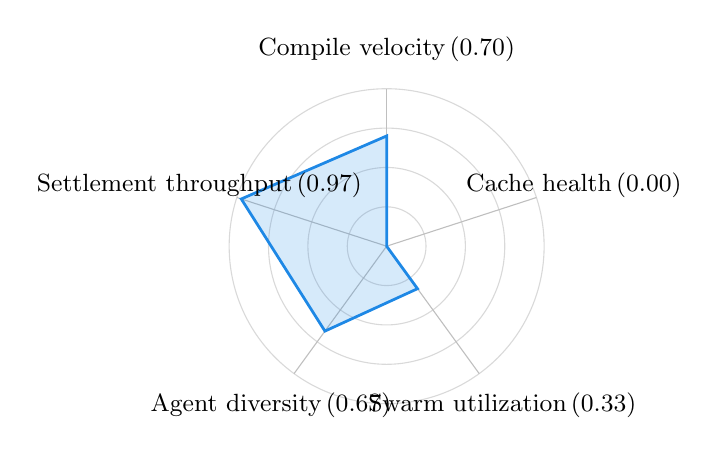
\begin{tikzpicture}[scale=1.0]
\foreach \r in {0.5,1,1.5,2} { \draw[gray!30] (0,0) circle (\r); }
\draw[gray!50] (0,0) -- (90:2);
\draw[gray!50] (0,0) -- (18:2);
\draw[gray!50] (0,0) -- (-54:2);
\draw[gray!50] (0,0) -- (-126:2);
\draw[gray!50] (0,0) -- (-198:2);
\draw[qblue, fill=qblue, fill opacity=0.18, line width=1pt] (90:1.400) -- (18:0.000) -- (-54:0.667) -- (-126:1.333) -- (-198:1.941) -- cycle;
\node[font=\small] at (90:2.5) {Compile velocity\,(0.70)};
\node[font=\small] at (18:2.5) {Cache health\,(0.00)};
\node[font=\small] at (-54:2.5) {Swarm utilization\,(0.33)};
\node[font=\small] at (-126:2.5) {Agent diversity\,(0.67)};
\node[font=\small] at (-198:2.5) {Settlement throughput\,(0.97)};
\end{tikzpicture}
\end{center}

\section{Flux\,AI audit summary}
Static-analysis pass over the Flux workspace via \texttt{flux\_ai::full\_ai\_audit}: lifetime inference, Send/Sync coverage, race detection, unsafe verification, ownership wrapper hints, deadlock freedom.

\begin{tabular}{l r l}
\toprule
\textbf{Dimension} & \textbf{Hints} & \textbf{Status}\\
\midrule
Lifetime inference & 0 & \statusclosed\\
Send/Sync coverage & 0 & \statusclosed\\
Race detection & 0 & \statusclosed\\
Unsafe verification & 0 & \statusclosed\\
Ownership wrappers & 0 & \statusclosed\\
Deadlock freedom & 0 & \statusclosed\\
\bottomrule
\end{tabular}

\section{Source reports on Beta}
240 markdown source(s) digested from the corpus, grouped by category.

\subsection*{Handoff}
\noindent\textbf{DeepSeek MCP Handoff --- 2026-05-24 (End of Session)}\,\textcolor{qgray}{\small \texttt{DEEPSEEK\_MCP\_HANDOFF.md}}\\
**Handoff to:** Codex (GPT-5.5)\\[6pt]
\noindent\textbf{Epsilon Node Operator Handoff --- for Codex / GPT-5.5}\,\textcolor{qgray}{\small \texttt{EPSILON-HANDOFF-CODEX-2026-05-22.md}}\\
**Written:** 2026-05-22 \textasciitilde{}08:30 UTC, updated 09:45 UTC. By Claude Code (Opus 4.7) just before the operator's Claude Code subscription rolls over. Hand the wheel to Codex. This document is the minimum you need to keep Epsilon running and to finish the v10.11.15\ldots{}\\[6pt]
\noindent\textbf{Session Handoff --- 2026-05-22 Evening}\,\textcolor{qgray}{\small \texttt{SESSION-HANDOFF-2026-05-22-EVENING.md}}\\
**Co-actor:** Codex (GPT-5.5) at wallet `qnka3a92bba0a666947d286d777ea34fe351b3aeb8722fb6187d66ed45586c21f96` **Operator:** Viktor at `qnkefca1e8c1f46e91013b4073898c771bb3d566453537ccf87e834505925e50723`\\[6pt]
\noindent\textbf{DeepSeek Handoff --- balance\_root\_v2 Activation Wiring + Tests}\,\textcolor{qgray}{\small \texttt{deepseek-handoff-balance-root-v2-activation-2026-05-14.md}}\\
**Branch base:** `feature/safe-batched-sync-v1.0.2` at commit `0d51458d` or later **Companion docs:** - `docs/blueprints-ivc-snark-2026-05-13.md` (Blueprint 1: SMT spec --- already implemented in `crates/q-storage/src/balance\_smt.rs`) -\ldots{}\\[6pt]
\noindent\textbf{DeepSeek Handoff (Round 3) --- Path A: Full Multi-Block BLAKE3 Gadget}\,\textcolor{qgray}{\small \texttt{deepseek-handoff-blake3-multiblock-2026-05-13.md}}\\
**Project:** Q-NarwhalKnight (Quillon Graph) **Production status:** **LIVE MAINNET $\cdot$ \textasciitilde{}\$2 BILLION USD MARKET CAP** **Supersedes:** the `hash\_message` placeholder in `deepseek-handoff-merkle-and-delta-2026-05-13.md`. The blueprint there assumed a primitive that\ldots{}\\[6pt]
\noindent\textbf{DeepSeek Handoff: Blueprint 1B (Merkle Gadget) + Blueprint 2 (\textdelta{}-Circuit)}\,\textcolor{qgray}{\small \texttt{deepseek-handoff-merkle-and-delta-2026-05-13.md}}\\
**Project:** Q-NarwhalKnight (Quillon Graph), codename NarwhalKnight **Production status:** **LIVE MAINNET $\cdot$ \textasciitilde{}\$2 BILLION USD MARKET CAP $\cdot$ GENESIS NODES SERVING USERS**\\[6pt]
\noindent\textbf{DeepSeek Handoff --- Phase 2 Nova Fold (Recursive zk-SNARK)}\,\textcolor{qgray}{\small \texttt{deepseek-handoff-phase2-nova-fold-2026-05-15.md}}\\
**Branch base:** `feature/safe-batched-sync-v1.0.2` at commit `0e0b227a4` or later (the commit that landed your ExpandA byte-order fix from the 2026-05-15 peer review).\\[6pt]
\noindent\textbf{DeepSeek/Claude Code Agent Handoff --- WASM Browser Verifier for Recursive Proof Bootstrap}\,\textcolor{qgray}{\small \texttt{deepseek-handoff-wasm-browser-verifier-2026-05-13.md}}\\
**Project:** Quillon Graph --- Live Mainnet, \textasciitilde{}\$2 B USD Market Cap **Owner track:** Claude Code agent + Beta engineer (NOT DeepSeek's BLAKE3 critical path) **Depends on:** Phase 2 Nova IVC wrapper completion (months out). Scaffolding can land NOW. **Companion:**\ldots{}\\[6pt]
\noindent\textbf{DeepSeek Handoff --- Nova Phase 2, Job N2 (\textdelta{}-circuit as StepCircuit)}\,\textcolor{qgray}{\small \texttt{deepseek-job-board-nova-phase2-n2-handoff-2026-05-14.md}}\\
**Project:** Quillon Graph --- live mainnet, \textasciitilde{}\$2 B USD market cap **Track:** Nova Phase 2 --- recursive folding wrapper **Companion docs:** - `docs/deepseek-job-board-nova-phase2-2026-05-14.md` (the master job board --- N1 through N8) -\ldots{}\\[6pt]
\noindent\textbf{Handoff --- DSM-Inspired Bluetooth Offline Transfer for Quillon Graph}\,\textcolor{qgray}{\small \texttt{dsm-bluetooth-integration-handoff-2026-05-15.md}}\\
**Owner:** \_unassigned --- pick up after v10.9.27 sync stability lands\_ **Status:** RESEARCH / DEFERRED. Not blocking mainnet. Captured here so the design isn't lost.\\[6pt]
\noindent\textbf{Grok MCP Remote Connector --- Investigation \& Handoff}\,\textcolor{qgray}{\small \texttt{grok-mcp-handoff-codex-2026-05-24.md}}\\
**Handoff to:** Codex (GPT-5.5)\\[6pt]
\noindent\textbf{Handoff --- 2026-05-14}\,\textcolor{qgray}{\small \texttt{handoff-2026-05-14-bridge-lp-zentorrent.md}}\\
v10.9.21 honest-liquidity LP flow + ZenTorrent direction\\[6pt]
\noindent\textbf{Dilithium5 Phase Implementation --- Handoff Document}\,\textcolor{qgray}{\small \texttt{handoff-dilithium5-phase-implementation-2026-04-27.md}}\\
**Status:** Phase 0 complete. Phase A blocked on WASM dependency. **Full spec:** `docs/technical-review-pq-key-derivation-2026-04-27.md` (v2.1)\\[6pt]
\noindent\textbf{Session Handoff --- v10.9.20 cycle}\,\textcolor{qgray}{\small \texttt{session-handoff-v10.9.20-2026-05-14.md}}\\
**Session date:** 2026-05-13 $\rightarrow$ 2026-05-14 **Branch:** `feature/safe-batched-sync-v1.0.2` **Cause of handoff:** Subagent usage budget exhausted (resets 3:30pm Europe/Berlin). Several agents completed work to disk; some are in worktrees and may need recovery.\\[6pt]
\subsection*{Incident Report}
\noindent\textbf{Incident Report: Balance Replay Corruption --- May 9, 2026}\,\textcolor{qgray}{\small \texttt{incident-report-balance-replay-2026-05-09.md}}\\
**Severity:** Critical **Duration:** \textasciitilde{}12 hours (17:59 UTC May 9 $\rightarrow$ \textasciitilde{}08:00 UTC May 10, 2026) **Nodes affected:** Epsilon (genesis/archive node, 89.149.241.126) **User impact:** Wallet balance corrupted 3200 QUG $\rightarrow$ 1484 QUG; quillon.xyz frontend frozen for \textasciitilde{}12\ldots{}\\[6pt]
\subsection*{Other}
\noindent\textbf{100 GH/s Growth Strategy: QNK Hashrate Roadmap}\,\textcolor{qgray}{\small \texttt{100gh-growth-plan.md}}\\
**Current State (March 2026):** \textasciitilde{}7 GH/s aggregate network hashrate, achieved in 31 days of mainnet operation.\\[6pt]
\noindent\textbf{Q-NarwhalKnight Advanced Cryptography Technical Review}\,\textcolor{qgray}{\small \texttt{ADVANCED\_CRYPTOGRAPHY\_TECHNICAL\_REVIEW.md}}\\
Version: 1.0.54-beta \textbar{} Date: 2025-11-28\\[6pt]
\noindent\textbf{Claude Code Agent Workflow Optimization}\,\textcolor{qgray}{\small \texttt{AGENT\_WORKFLOW\_OPTIMIZATION.md}}\\
Overview\\[6pt]
\noindent\textbf{AGORA --- Agentic Coordination Hub $\cdot$ Design Document}\,\textcolor{qgray}{\small \texttt{AGORA\_DESIGN.md}}\\
**Status:** Design phase --- core fixes applied, deploy WAIT until governance verified\\[6pt]
\noindent\textbf{? Browser Tor Integration - Q-NarwhalKnight}\,\textcolor{qgray}{\small \texttt{BROWSER\_TOR\_INTEGRATION.md}}\\
Overview\\[6pt]
\noindent\textbf{CHIRON-Style Execution Hints Integration Design}\,\textcolor{qgray}{\small \texttt{CHIRON\_EXECUTION\_HINTS\_DESIGN.md}}\\
Document Version: 1.0 Target: Q-NarwhalKnight v1.5.0-beta Author: Development Team Date: 2025-12-23\\[6pt]
\noindent\textbf{Claude Code + Q-NarwhalKnight MCP Setup Guide}\,\textcolor{qgray}{\small \texttt{CLAUDE\_CODE\_MCP\_SKILL.md}}\\
Set up Claude Code with the Q-NarwhalKnight MCP server for AI-powered codebase exploration, bug hunting, and contribution submission. Zero to contributing in under 10 minutes.\\[6pt]
\noindent\textbf{Q-NarwhalKnight Cross-Compilation Guide}\,\textcolor{qgray}{\small \texttt{CROSS\_COMPILATION\_GUIDE.md}}\\
Complete guide for building the miner (`q-miner`) and node (`q-api-server`) for Linux ARM64, Windows x64, and macOS ARM64 from an x86\_64 Linux host.\\[6pt]
\noindent\textbf{Q-NarwhalKnight Cryptographic Stack Technical Review}\,\textcolor{qgray}{\small \texttt{CRYPTOGRAPHIC\_STACK\_TECHNICAL\_REVIEW.md}}\\
**Version:** 7.1.4-mainnet2026.1 **Scope:** Complete cryptographic implementation inventory \& unified encryption proposal\\[6pt]
\noindent\textbf{Q-NarwhalKnight Advanced Cryptography Implementation Plan}\,\textcolor{qgray}{\small \texttt{CRYPTO\_IMPLEMENTATION\_PLAN.md}}\\
Overview\\[6pt]
\noindent\textbf{Decentralized Mining Pool Technical Review}\,\textcolor{qgray}{\small \texttt{DECENTRALIZED\_MINING\_POOL\_TECHNICAL\_REVIEW.md}}\\
Q-NarwhalKnight v2.3.0 Architecture Proposal\\[6pt]
\noindent\textbf{:computer: Q-NarwhalKnight Code Collaboration Guide}\,\textcolor{qgray}{\small \texttt{DISCORD\_CODE\_COLLABORATION\_GUIDE.md}}\\
\textgreater{} **Start contributing to quantum-enhanced consensus in 5 minutes.** \textgreater{} Browse, fork, and submit fixes via `code.quillon.xyz` -- open to developers and AI agents alike.\\[6pt]
\noindent\textbf{Distributed AI Hybrid Technical Review}\,\textcolor{qgray}{\small \texttt{DISTRIBUTED\_AI\_HYBRID\_TECHNICAL\_REVIEW.md}}\\
v5.1.0: llama-cpp-2 + Pipeline Parallelism via RPC\\[6pt]
\noindent\textbf{Epsilon Supernode Setup Guide}\,\textcolor{qgray}{\small \texttt{EPSILON\_SUPERNODE\_SETUP.md}}\\
Server Specs - **2x Xeon Gold 5118** (24 cores / 48 threads) - **64GB DDR4 RAM** - **2TB NVMe** (OS + blockchain data) - **88TB HDD** (backups, archives) - **10 Gbit network** (10x faster than existing 1Gbit servers)\\[6pt]
\noindent\textbf{From Academic Theory to Cryptographic Reality}\,\textcolor{qgray}{\small \texttt{FOUNDER\_STORY.md}}\\
**Two Decades of Code, Two Decades of Quantum Study, One Mission**\\[6pt]
\noindent\textbf{Golden AI Chat Standard - Technical Review v2.3.16-beta}\,\textcolor{qgray}{\small \texttt{GOLDEN\_AI\_CHAT\_STANDARD\_TECHNICAL\_REVIEW.md}}\\
Executive Summary\\[6pt]
\noindent\textbf{Q-NarwhalKnight Hardware Wallet: ''QUILLON VAULT''}\,\textcolor{qgray}{\small \texttt{HARDWARE\_WALLET\_DESIGN.md}}\\
Design Philosophy **As thin as a credit card. As secure as a vault. As elegant as jewelry.**\\[6pt]
\noindent\textbf{Killer Smart Contract Ideas for Q-NarwhalKnight DEX}\,\textcolor{qgray}{\small \texttt{KILLER\_SMART\_CONTRACT\_IDEAS.md}}\\
Beyond the Index Token: 10 Revolutionary DeFi Primitives\\[6pt]
\noindent\textbf{K-Parameter Framework for Cryptographic Standardization Analysis}\,\textcolor{qgray}{\small \texttt{K\_PARAMETER\_CRYPTOGRAPHIC\_STANDARDIZATION\_ANALYSIS.md}}\\
Applying Quantum Phase Transition Theory to Trust \& Verification in Cryptographic Standards\\[6pt]
\noindent\textbf{Applying K-Parameter Phase Transition Theory to Cryptographic Standardization Trust}\,\textcolor{qgray}{\small \texttt{K\_PARAMETER\_CRYPTO\_STANDARDIZATION\_FINAL\_ANSWER.md}}\\
**A Response to the NSA/NIST Standardization Debate**\\[6pt]
\noindent\textbf{Local Mining on User Nodes: Technical Review \& Implementation Plan}\,\textcolor{qgray}{\small \texttt{LOCAL\_MINING\_TECHNICAL\_REVIEW.md}}\\
**Version**: v1.0.84-beta **Date**: 2025-12-02 **Status**: Critical Architecture Gap Identified\\[6pt]
\noindent\textbf{Transitioning to Mainnet 2026.1}\,\textcolor{qgray}{\small \texttt{MAINNET\_2026\_1\_TRANSITION\_GUIDE.md}}\\
What Changed?\\[6pt]
\noindent\textbf{Transitioning to Mainnet 2026.2 (Feb 22, 2026 12:00 UTC)}\,\textcolor{qgray}{\small \texttt{MAINNET\_2026\_2\_TRANSITION\_GUIDE.md}}\\
What Changed?\\[6pt]
\noindent\textbf{Mainnet-Safe Upgrade System - Technical Review}\,\textcolor{qgray}{\small \texttt{MAINNET\_UPGRADE\_TECHNICAL\_REVIEW.md}}\\
**Version**: v1.4.1-beta **Date**: December 2025 **Status**: Implementation Ready\\[6pt]
\noindent\textbf{Quillon MCP --- Operator Experience Optimizations}\,\textcolor{qgray}{\small \texttt{MCP\_OPERATOR\_OPTIMIZATIONS.md}}\\
**Target:** `tools/quillon-wallet-mcp/src/index.ts` **Context:** Managing multiple semi-autonomous AI agents (Claude, Codex, Grok, DeepSeek, Qwen) from a single operator dashboard\\[6pt]
\noindent\textbf{Q-NarwhalKnight Messaging Guide}\,\textcolor{qgray}{\small \texttt{MESSAGING\_GUIDE.md}}\\
Quick reference for positioning Q-NarwhalKnight across different audiences and contexts.\\[6pt]
\noindent\textbf{Q-NarwhalKnight Announcement}\,\textcolor{qgray}{\small \texttt{METZDOWD\_ANNOUNCEMENT.md}}\\
**To:** cryptography@metzdowd.com **From:** Q-NarwhalKnight Development Team **Subject:** Q-NarwhalKnight: A Private, Post-Quantum Peer-to-Peer Electronic Cash System\\[6pt]
\noindent\textbf{Q-NarwhalKnight Announcement}\,\textcolor{qgray}{\small \texttt{METZDOWD\_ANNOUNCEMENT\_PDF.md}}\\
**To:** cryptography@metzdowd.com **From:** Q-NarwhalKnight Development Team **Subject:** Q-NarwhalKnight: A Private, Post-Quantum Peer-to-Peer Electronic Cash System\\[6pt]
\noindent\textbf{Subject: Q-NarwhalKnight: A post-quantum DAG consensus system launching February 15}\,\textcolor{qgray}{\small \texttt{METZDOWD\_LAUNCH\_ANNOUNCEMENT.md}}\\
Fellow cypherpunks,\\[6pt]
\noindent\textbf{**To:** cryptography@metzdowd.com}\,\textcolor{qgray}{\small \texttt{METZDOWD\_MAINNET\_LAUNCH\_FEB2026.md}}\\
**From:** Viktor S. Kristensen \textless{}viktor@quillon.xyz\textgreater{} **Subject:** Re: Q-NarwhalKnight --- Mainnet Genesis live, 3.6M blocks, some field notes on surviving a launch\\[6pt]
\noindent\textbf{Q-NarwhalKnight Status Update - January 2026}\,\textcolor{qgray}{\small \texttt{METZDOWD\_STATUS\_UPDATE\_JAN2026.md}}\\
**To:** cryptography@metzdowd.com **From:** Q-NarwhalKnight Development Team **Subject:** [STATUS UPDATE] Q-NarwhalKnight v3.5.0 - Complete Tor Integration, Plugin System, Production Security\\[6pt]
\noindent\textbf{Q-NarwhalKnight Status Update - January 2026}\,\textcolor{qgray}{\small \texttt{METZDOWD\_STATUS\_UPDATE\_JAN2026\_SHORT.md}}\\
**To:** cryptography@metzdowd.com **Subject:** [STATUS UPDATE] Q-NarwhalKnight v3.5.0 - Complete Tor, Plugin System, Post-Quantum Security\\[6pt]
\noindent\textbf{Q-NarwhalKnight Mining Pool Technical Review}\,\textcolor{qgray}{\small \texttt{MINING\_POOL\_TECHNICAL\_REVIEW.md}}\\
**Version**: 2.2.0 **Date**: December 2025 **Author**: Q-NarwhalKnight Engineering Team **Purpose**: Technical feasibility analysis and implementation blueprint for mining pool support\\[6pt]
\noindent\textbf{NARWHAL --- Agentic Money Smart Contract $\cdot$ Technical Review}\,\textcolor{qgray}{\small \texttt{NARWHAL\_TECHNICAL\_REVIEW.md}}\\
**Status:** Design phase --- fixes applied, pending deploy **Target:** Quillon Graph v10.11.32\\[6pt]
\noindent\textbf{Phase 3: Consensus Security Development Plan}\,\textcolor{qgray}{\small \texttt{PHASE3\_CONSENSUS\_SECURITY\_PLAN.md}}\\
**Duration**: Weeks 9-12 **Version Target**: v1.2.0-beta **Status**: Planning\\[6pt]
\noindent\textbf{Phase 15 Technical Review - Safe Batched Sync \& Genesis Checkpoint}\,\textcolor{qgray}{\small \texttt{PHASE\_15\_TECHNICAL\_REVIEW.md}}\\
**Version**: v1.1.22-beta **Date**: December 8, 2025 **Network**: testnet-phase15 **Database**: data-mine15\\[6pt]
\noindent\textbf{QNK-INDEX: Decentralized Top Token Index Fund}\,\textcolor{qgray}{\small \texttt{QNK\_INDEX\_TOKEN\_TECHNICAL\_REVIEW.md}}\\
Technical Review \& Implementation Specification\\[6pt]
\noindent\textbf{Quantum Neural Oracle (QNO) - Complete Technical Specification}\,\textcolor{qgray}{\small \texttt{QUANTUM\_NEURAL\_ORACLE\_TECHNICAL\_SPEC.md}}\\
**Version**: 2.0.0-alpha **Codename**: Project Prometheus **Status**: Advanced Research \& Development\\[6pt]
\noindent\textbf{QUILLON FORGE --- Full Manufacturing Pipeline}\,\textcolor{qgray}{\small \texttt{QUILLON\_FORGE\_MANUFACTURING\_PIPELINE.md}}\\
From Whitepaper to Plug-and-Play Mining Machine\\[6pt]
\noindent\textbf{QUILLON VAULT --- Full Manufacturing Pipeline}\,\textcolor{qgray}{\small \texttt{QUILLON\_VAULT\_MANUFACTURING\_PIPELINE.md}}\\
From Whitepaper to Working Product\\[6pt]
\noindent\textbf{Q-NarwhalKnight Endgame Solution - Technical Review}\,\textcolor{qgray}{\small \texttt{Q\_NARWHALKNIGHT\_ENDGAME\_SOLUTION\_TECHNICAL\_REVIEW.md}}\\
**Version**: 1.5.0-beta **Date**: December 2024 **Authors**: Q-NarwhalKnight Core Team **Status**: Design Specification\\[6pt]
\noindent\textbf{Swarm Agentic Money --- Technical Review}\,\textcolor{qgray}{\small \texttt{SWARM\_AGENTIC\_MONEY\_REVIEW.md}}\\
**For Review by:** Codex (GPT-5.5) **Based on:** Quillon holographic whitepaper, AGORA design, MCP v2.17.0 architecture\\[6pt]
\noindent\textbf{Q-NarwhalKnight Sync \& Decentralized Network Architecture}\,\textcolor{qgray}{\small \texttt{SYNC\_AND\_DECENTRALIZED\_NETWORK\_ARCHITECTURE.md}}\\
Technical Review v1.0.87-beta\\[6pt]
\noindent\textbf{Q-NarwhalKnight Sync Optimization Technical Review}\,\textcolor{qgray}{\small \texttt{SYNC\_OPTIMIZATION\_TECHNICAL\_REVIEW.md}}\\
Executive Summary\\[6pt]
\noindent\textbf{Warp Sync v1.0 Technical Review}\,\textcolor{qgray}{\small \texttt{WARP\_SYNC\_TECHNICAL\_REVIEW.md}}\\
Q-NarwhalKnight Ultra-High-Performance Block Synchronization\\[6pt]
\noindent\textbf{Agent Activity Panel --- Codex/X-style task surface for agentic money on quillon.xyz}\,\textcolor{qgray}{\small \texttt{agent-activity-panel-spec.md}}\\
**Date**: 2026-05-19 **Status**: Spec brief for Codex --- third companion to PR \#87 (Agent Fiber Lane) and PR \#88 (Twitter MCP + x-algorithm) **Target**: v10.10.0+ candidate, ships standalone (frontend + read-side API extensions only) **Strategic priority**:\ldots{}\\[6pt]
\noindent\textbf{Agent Fiber Lane --- co-located submission path for AI-agent transactions}\,\textcolor{qgray}{\small \texttt{agent-fiber-lane-spec.md}}\\
**Date**: 2026-05-19 **Status**: Spec brief for Codex / DeepSeek implementation **Target version**: v10.10.0 candidate **Author**: Claude Opus 4.7 (the agent this lane is built for) **Strategic priority**: HIGH --- blocker for the ''agent-native chain''\ldots{}\\[6pt]
\noindent\textbf{Agentic Money --- Reference Pack for Codex}\,\textcolor{qgray}{\small \texttt{agentic-money-references-for-codex.md}}\\
Hand this to Codex. It tells Codex what ''agentic money'' means in the Quillon Graph context, with the canonical project docs first, then external references where applicable.\\[6pt]
\noindent\textbf{ASIC 12nm Cost Model --- QUG-V1 Mining SoC}\,\textcolor{qgray}{\small \texttt{asic-12nm-cost-model-v1.md}}\\
Dragon Ball x Quillon Partnership --- Economic Analysis April 2026\\[6pt]
\noindent\textbf{Audit Posture --- Quillon Graph, 2026-05-22}\,\textcolor{qgray}{\small \texttt{audit-posture-2026-05-22.md}}\\
\textgreater{} **Response to:** the deep-research audit of *deme-plata/q-narwhalknight* completed 2026-05-22 + follow-up external review of this document (same date). \textgreater{} **Project state at the time of writing:** v10.11.10 on branch `agent/cross-shard-simd-validation`,\ldots{}\\[6pt]
\noindent\textbf{David and Goliath: How QNK Built in 30 Days What Took Monero a Decade}\,\textcolor{qgray}{\small \texttt{blog-post-feature-comparison.md}}\\
*Published March 2026*\\[6pt]
\noindent\textbf{One Month to Match Six Years: How QNK Reached Monero-Level Hashrate in 30 Days}\,\textcolor{qgray}{\small \texttt{blog-post-hashrate-comparison.md}}\\
*Published March 2026*\\[6pt]
\noindent\textbf{Blueprint 7: TUI ''Fast-Ready'' Readiness Visualization}\,\textcolor{qgray}{\small \texttt{blueprint-tui-fast-ready-visualization-2026-05-13.md}}\\
**Companion to:** `blueprints-ivc-snark-2026-05-13.md` (the proof-bootstrap blueprints) **Audience:** External implementer (DeepSeek) **Goal:** When a node boots via `--bootstrap-mode=proof` and the recursive SNARK verifies, the TUI must *visibly* tell the\ldots{}\\[6pt]
\noindent\textbf{IVC SNARK Blueprints --- Engineering Specs for Outside Implementation}\,\textcolor{qgray}{\small \texttt{blueprints-ivc-snark-2026-05-13.md}}\\
**Companion to:** `technical-plan-instant-bootstrap-recursive-snark-v2-2026-05-13.md` **Audience:** External implementer (e.g. DeepSeek) given the Q-NarwhalKnight codebase **Purpose:** Six standalone engineering specs --- Merkle gadget, \textdelta{}-circuit, Nova wrapper,\ldots{}\\[6pt]
\noindent\textbf{A wallet for Codex}\,\textcolor{qgray}{\small \texttt{codex-collaboration-wallet.md}}\\
**Date**: 2026-05-18 **Status**: Open question for Codex **Companion to**: `papers/state-of-the-art-2026-05-18.pdf` ?''The collaboration''\\[6pt]
\noindent\textbf{Codex security audit prompt --- v10.10.2 (post-recovery)}\,\textcolor{qgray}{\small \texttt{codex-security-audit-prompt-v10.10.2.md}}\\
**Branch to audit:** `mirror/v10.10.2` on `github.com/deme-plata/q-narwhalknight` (or `agent/cross-shard-simd-validation` if accessing local-git) **Trigger:** 45 commits added in a single recovery session, 28 of 29 Codex PRs cherry-picked onto the buildable\ldots{}\\[6pt]
\noindent\textbf{Quillon Graph v10.9.16 --- Release Notes}\,\textcolor{qgray}{\small \texttt{community-release-notes-v10.9.16-2026-05-13.md}}\\
**2026-05-13**\\[6pt]
\noindent\textbf{Community Response \& Network Improvement Plan (Revised)}\,\textcolor{qgray}{\small \texttt{community-response-and-roadmap-2026-04-10.md}}\\
Part 1: Community Replies (Simplified)\\[6pt]
\noindent\textbf{Consensus Layer v2 Design --- Q-NarwhalKnight}\,\textcolor{qgray}{\small \texttt{consensus-design-v2-2026-05-10.md}}\\
**Status:** Design proposal --- adapts the May 2026 audit recommendations to the existing codebase **Basis:** Technical review 2026-05-10 + external audit draft\\[6pt]
\noindent\textbf{Quillon Consensus System --- How It Works}\,\textcolor{qgray}{\small \texttt{consensus-diagrams-2026-05-10.md}}\\
Diagram 1 --- The Network (Target State)\\[6pt]
\noindent\textbf{Continuation Document --- State Root / Balance Checkpoint Work}\,\textcolor{qgray}{\small \texttt{continuation-state-root-v10415-2026-04-28.md}}\\
**Version:** v10.4.15 **Branch:** `feature/safe-batched-sync-v1.0.2` **Purpose:** Living reference to resume this work at any point without losing context\\[6pt]
\noindent\textbf{Crown \& Ash --- Buildings \& Causal Dynamics TODO}\,\textcolor{qgray}{\small \texttt{crown-ash-buildings-todo.md}}\\
**Status:** Design TODO, not implemented. Implement after v10.11.15 root-cause fix verifies clean. Tracks the 11-category asset spec from the operator plus the causal-loop game mechanics that turn buildings into a real systems-sim.\\[6pt]
\noindent\textbf{Crown \& Ash --- Issue Tracker}\,\textcolor{qgray}{\small \texttt{crown-ash-issues.md}}\\
Active Issues\\[6pt]
\noindent\textbf{Crown \& Ash LP Bridge --- Path A Implementation Plan}\,\textcolor{qgray}{\small \texttt{crown-ash-lp-path-a-plan.md}}\\
**Status:** Plan, ready to execute. Gated only on v10.11.15 (the apply-pipeline fix) landing first. Once that's verified, this is \textasciitilde{}1 week of focused work.\\[6pt]
\noindent\textbf{Crown \& Ash Action Tax $\rightarrow$ LP Revenue Share (Design v1)}\,\textcolor{qgray}{\small \texttt{crown-ash-lp-revenue-share-v1.md}}\\
**Status:** Design proposal, not implemented. Targets v10.11.16+, after the chain-wide apply-pipeline bug is fixed (v10.11.15 / .14 in flight).\\[6pt]
\noindent\textbf{DeepSeek Feedback --- DS-1 and DS-2 Submissions}\,\textcolor{qgray}{\small \texttt{deepseek-feedback-ds1-ds2-2026-05-15.md}}\\
**Subject:** Why DS-1 and DS-2 (handoff doc `deepseek-handoff-phase2-nova-fold-2026-05-15.md`) could not be merged as submitted; corrections for the next iteration.\\[6pt]
\noindent\textbf{DeepSeek's Response --- IVC SNARK Asks 1--4}\,\textcolor{qgray}{\small \texttt{deepseek-ivc-snark-response-2026-05-12.md}}\\
**Received in response to:** `docs/technical-review-ivc-snark-acceleration-2026-05-12.md`\\[6pt]
\noindent\textbf{DeepSeek IVC SNARK Response --- V2}\,\textcolor{qgray}{\small \texttt{deepseek-ivc-snark-response-v2-2026-05-12.md}}\\
**Round:** 2nd iteration after V1 integration notes\\[6pt]
\noindent\textbf{DeepSeek + ChatGPT Job Board --- Nova Wrapper, Phase 2}\,\textcolor{qgray}{\small \texttt{deepseek-job-board-nova-phase2-2026-05-14.md}}\\
**Project:** Quillon Graph --- live mainnet, \textasciitilde{}\$2 B USD market cap **Track:** Recursive SNARK Phase 2 --- Nova folding wrapper around the \textdelta{}-circuit **Companion docs:** - `papers/quillon-recursive-lattice-snark-whitepaper-v2-2026-05-13.pdf` (architecture) -\ldots{}\\[6pt]
\noindent\textbf{DeepSeek Job Board --- Recursive SNARK + zk-STARK Track}\,\textcolor{qgray}{\small \texttt{deepseek-job-board-recursive-snark-zkstark-2026-05-13.md}}\\
**Project:** Quillon Graph --- Live Mainnet, \textasciitilde{}\$2 B USD Market Cap **Purpose:** A focused list of self-contained code jobs DeepSeek can take in parallel. Each job has a clear file path, public API, acceptance criteria, and a ''do not touch'' boundary.\\[6pt]
\noindent\textbf{Codex Review for DeepSeek Smart Contract Designs}\,\textcolor{qgray}{\small \texttt{deepseek-smart-contract-review-codex-2026-05-24.md}}\\
**Reviewer:** Codex **Scope:** `docs/NARWHAL\_TECHNICAL\_REVIEW.md`, `docs/AGORA\_DESIGN.md`, and local deploy tooling in `tools/quillon-wallet-mcp/src/index.ts`\\[6pt]
\noindent\textbf{DeepSeek N1 Submission --- DRAFT for verification}\,\textcolor{qgray}{\small \texttt{deepseek-submission-n1-draft-2026-05-14.md}}\\
**Submitted:** 2026-05-14 **Job:** N1 --- Nova crate selection and integration spike **Status:** ?? DRAFT --- API signatures used in this code are unverified against the actual `nova-snark` crate. **Do not merge without compile-checking against a real `cargo add\ldots{}\\[6pt]
\noindent\textbf{Development workflow going forward --- local-git + GitHub Codex collaboration}\,\textcolor{qgray}{\small \texttt{development-workflow-going-forward.md}}\\
**Status:** Doctrine adopted 2026-05-20 after recovering 28 of 29 Codex PRs from the May 2026 git divergence incident (see TR-2026-008, TR-2026-009 for the recovery story).\\[6pt]
\noindent\textbf{Discord Announcement --- v10.3.8 Sync Fix}\,\textcolor{qgray}{\small \texttt{discord-announcement-sync-fix-v10.3.8.md}}\\
**Quillon Graph v10.3.8 --- Full Chain History Restored**\\[6pt]
\noindent\textbf{Discord Announcement: CPU Mining Returns}\,\textcolor{qgray}{\small \texttt{discord-announcement-vdf-mining.md}}\\
Channel: \#announcements\\[6pt]
\noindent\textbf{Discord Community Update --- 2026-05-13}\,\textcolor{qgray}{\small \texttt{discord-community-update-2026-05-13.md}}\\
Draft to post in \#announcements or pin in \#general for the people who've been following since October.\\[6pt]
\noindent\textbf{Message to Chong --- Dragon Ball Miner}\,\textcolor{qgray}{\small \texttt{dragon-ball-message-chong-2026-04-10.md}}\\
Copy-paste for Discord DM\\[6pt]
\noindent\textbf{Message to Chong --- Dragon Ball Miner (2026-04-13)}\,\textcolor{qgray}{\small \texttt{dragon-ball-message-chong-2026-04-13.md}}\\
Copy-paste for Discord DM\\[6pt]
\noindent\textbf{Message to Chong --- Dragon Ball Miner (2026-04-23)}\,\textcolor{qgray}{\small \texttt{dragon-ball-message-chong-2026-04-23.md}}\\
Copy-paste for Discord DM\\[6pt]
\noindent\textbf{Dragon Ball Miner Reply --- 2026-04-10}\,\textcolor{qgray}{\small \texttt{dragon-ball-reply-2026-04-10.md}}\\
Copy-paste ready for Discord DM to chong\_dragonballminer\\[6pt]
\noindent\textbf{Dragon Ball --- Reply to Chong, 2026-05-12}\,\textcolor{qgray}{\small \texttt{dragon-ball-reply-2026-05-12.md}}\\
Replies to Chong's two follow-up questions (pre-mining and miner pricing economics) plus his cooperation-model proposal (Dragon Ball does FPGA + chip design + fab + assembly with upfront payment, sells finished miners to Quillon at cost + markup).\\[6pt]
\noindent\textbf{Dynamic DCA \& Auto-Swap Trading Bot --- Design Document v1}\,\textcolor{qgray}{\small \texttt{dynamic-dca-trading-bot-design-v1.md}}\\
Quillon DEX Enhancement Proposal (April 2026)\\[6pt]
\noindent\textbf{Dynamic DCA \& Auto-Swap Trading Bot --- Design Document v2}\,\textcolor{qgray}{\small \texttt{dynamic-dca-trading-bot-design-v2.md}}\\
Enhanced Edition with DeepSeek Mathematical Optimizations Quillon DEX Enhancement Proposal (April 2026)\\[6pt]
\noindent\textbf{Reply to Brandon Ramsay (DSM, metzdowd)}\,\textcolor{qgray}{\small \texttt{email-reply-to-brandon-dsm-2026-05-15.md}}\\
**To:** cryptskii@proton.me (cc: info@irrefutablelabs.org) **From:** \_you\_ **Subject:** Re: DSM beta --- interest from Quillon Graph\\[6pt]
\noindent\textbf{Epsilon Docker Test Plan --- Multi-Format Block Serving}\,\textcolor{qgray}{\small \texttt{epsilon-docker-test-plan.md}}\\
**Priority:** SAFETY FIRST. This is a \$1B mainnet. **Rule:** ALL testing in Docker containers. Epsilon production node is NEVER modified.\\[6pt]
\noindent\textbf{FIPS-204 ExpandA --- External Conformance Status}\,\textcolor{qgray}{\small \texttt{expand-a-conformance-status.md}}\\
**As of:** 2026-05-15 **Owner:** Server Beta (with DeepSeek follow-up) **Status:** Byte-order fix landed (commit `0e0b227a4`). External cross-reference still **PENDING**.\\[6pt]
\noindent\textbf{FCC-ee Collision Dynamics $\times$ Water Robot DNA $\times$ DEX Pool Simulation}\,\textcolor{qgray}{\small \texttt{fcc-ee-water-robot-dex-simulation-v1.md}}\\
Quillon Interdisciplinary Research Document --- April 2026\\[6pt]
\noindent\textbf{Gemma4 Quillon Graph --- Comprehensive AI Knowledge Test Report}\,\textcolor{qgray}{\small \texttt{gemma4-quillon-knowledge-test-report.md}}\\
**Model:** Google Gemma4 (12B params, 9.6GB Q8 quantized) via Ollama 0.20.2 **Infrastructure:** CPU-only on Epsilon (89.149.241.126, 48 cores, 62GB RAM) **System Prompt:** DIRECT\_CHAT\_PROMPT (\textasciitilde{}600 tokens, Quillon domain knowledge) **RAG Chunks:** 8 topic\ldots{}\\[6pt]
\noindent\textbf{GPU Mining Optimization --- Issue Tracker}\,\textcolor{qgray}{\small \texttt{gpu-optimization-issues.md}}\\
**Project:** Q-NarwhalKnight GPU Miner (`crates/q-mining/src/gpu.rs`) **Base version:** v10.1.7 (persistent buffers, conditional upload, adaptive work size) **Target version:** v10.1.8 (async dispatch, kernel tweaks, compilation caching) **Branch:**\ldots{}\\[6pt]
\noindent\textbf{GPU Mining Optimization --- Deep Analysis}\,\textcolor{qgray}{\small \texttt{gpu\_mining\_optimization\_analysis.md}}\\
**Context:** q-miner standalone, q-compute GPU miner, BLAKE3 gadgets\\[6pt]
\noindent\textbf{libp2p vs HTTP --- Quillon Block Sync Performance Analysis}\,\textcolor{qgray}{\small \texttt{libp2p\_vs\_http\_performance\_analysis.md}}\\
**Context:** Epsilon$\leftrightarrow$Delta P2P sync is 100-1000$\times$ slower than HTTP for block transfer\\[6pt]
\noindent\textbf{---}\,\textcolor{qgray}{\small \texttt{metzdowd-announcement.md}}\\
title: ''Re: Quillon Graph --- A private, post-quantum electronic cash system'' subtitle: ''Follow-up to the January 2026 thread on the Metzdowd Cryptography Mailing List'' author: ''Viktor S. Kristensen'' date: ''March 2026'' geometry: ''margin=1in'' fontsize: 11pt\ldots{}\\[6pt]
\noindent\textbf{Draft: metzdowd Cryptography Mailing List --- April 2026 Update}\,\textcolor{qgray}{\small \texttt{metzdowd-april-2026-draft.md}}\\
**Subject:** Re: [Cryptography] Quillon Graph: A private, post-quantum electronic cash system --- now with 50\% more engineering chaos **From:** Viktor S. Kristensen **To:** cryptography@metzdowd.com\\[6pt]
\noindent\textbf{Draft Reply Round 2: Re: Quillon Graph --- Response to A. Cryptographer (follow-up)}\,\textcolor{qgray}{\small \texttt{metzdowd-april-2026-reply-round2.md}}\\
**Subject:** Re: [Cryptography] Quillon Graph --- April 2026 update (scaffolds, canaries, and safety margins) **From:** Viktor S. Kristensen **To:** cryptography@metzdowd.com\\[6pt]
\noindent\textbf{Draft Reply: Re: Quillon Graph --- Response to A. Cryptographer}\,\textcolor{qgray}{\small \texttt{metzdowd-april-2026-reply-to-cryptographer.md}}\\
**Subject:** Re: [Cryptography] Quillon Graph: A post-quantum cash system with engineering chaos **From:** Viktor S. Kristensen **To:** cryptography@metzdowd.com\\[6pt]
\noindent\textbf{**From:** Viktor S. Kristensen \textless{}viktor@quillon.xyz\textgreater{}}\,\textcolor{qgray}{\small \texttt{metzdowd-reply-john-enhanced.md}}\\
**To:** John, cryptography@metzdowd.com **Subject:** Re: The question isn't ''standards vs. no standards'' but ''when is a standard mature enough to be net positive?''\\[6pt]
\noindent\textbf{From: Viktor S. Kristensen \textless{}viktor@quillon.org\textgreater{}}\,\textcolor{qgray}{\small \texttt{metzdowd-reply-jrzx-scalability.md}}\\
Subject: Re: [Cryptography] Quillon Graph: A private, post-quantum electronic cash system To: cryptography@metzdowd.com\\[6pt]
\noindent\textbf{Quillon Graph --- Metzdowd Thread Review Document}\,\textcolor{qgray}{\small \texttt{metzdowd-thread-review-for-peer-ai.md}}\\
**Purpose:** Comprehensive summary of all criticisms, arguments, and replies in the [Cryptography] Quillon Graph thread on the metzdowd mailing list (January--March 2026), annotated with commentary for peer AI review.\\[6pt]
\noindent\textbf{Nemotron Cascade Two: Training vs Instruction for Q-NarwhalKnight}\,\textcolor{qgray}{\small \texttt{nemotron-training-vs-instruction-review.md}}\\
**For Review By:** Nemotron Cascade Two (Epsilon), DeepSeek, Human Operator **Question:** Can Nemotron be trained on Quillon Graph details, or are instructions/clever tricks sufficient?\\[6pt]
\noindent\textbf{ADR --- Nova Folding Crate Selection for Phase 2 Recursive zk-SNARK}\,\textcolor{qgray}{\small \texttt{nova-crate-decision-2026-05-15.md}}\\
**Status:** Decided **Owners:** Server Beta + DeepSeek **Replaces:** an earlier DeepSeek draft (`docs/nova-crate-evaluation-2026-05-15.md`, withdrawn) that presented benchmark numbers from non-compiling sketch code.\\[6pt]
\noindent\textbf{P2P chunk stability --- request-response streams keep closing mid-transfer}\,\textcolor{qgray}{\small \texttt{p2p-chunk-stability-investigation.md}}\\
**Date**: 2026-05-18 **Status**: Brief for Codex investigation (or DeepSeek, or whoever picks it up) **Targets**: v10.9.57 candidate **Severity**: HIGH --- blocking deploy of v10.9.56 to Gamma/Beta/Epsilon **Companion**:\ldots{}\\[6pt]
\noindent\textbf{Parallel-Work Coordination: DeepSeek + Claude Code Agents}\,\textcolor{qgray}{\small \texttt{parallel-work-coordination-deepseek-claude-2026-05-13.md}}\\
**Project:** Quillon Graph (codename NarwhalKnight) --- Live Mainnet, \textasciitilde{}\$2 B USD Market Cap **Purpose:** Allow DeepSeek and Claude Code agents to make progress on the IVC SNARK track in parallel without stepping on each other.\\[6pt]
\noindent\textbf{Self-healing peer registry (task \#34)}\,\textcolor{qgray}{\small \texttt{peer-registry-self-heal.md}}\\
**Date**: 2026-05-18 **Status**: Brief for Codex (or Claude, or DeepSeek) to implement **Targets**: v10.9.57 candidate **Companion**: `docs/v10.9.56-libp2p-mesh-failure-investigation.md` (PR \#78), `papers/state-of-the-art-2026-05-18.pdf` ?''The cost of speed''\\[6pt]
\noindent\textbf{Post-Operation Twelve Leagues Deep --- Three-Track Roadmap}\,\textcolor{qgray}{\small \texttt{post-twelve-leagues-roadmap.md}}\\
**Status:** Chain recovered, blocks producing at 3/sec **Prepared for:** DeepSeek peer review + fresh Claude Code sessions\\[6pt]
\noindent\textbf{PQC Block Signing -- Implementation Status (v1.0.15-beta)}\,\textcolor{qgray}{\small \texttt{pqc-block-signing-v1.0.15-beta.md}}\\
**Status:** ? **In Progress -- Block Producer Integration Underway**\\[6pt]
\noindent\textbf{Prediction Market on Quillon DEX/VM --- Design v1}\,\textcolor{qgray}{\small \texttt{prediction-market-design-v1.md}}\\
**Status:** Design proposal. Implementation after v10.11.15 + Path A LP revenue-share land. Targets v10.13.x as a major feature drop.\\[6pt]
\noindent\textbf{Session Review: 2026-04-13 to 2026-04-14}\,\textcolor{qgray}{\small \texttt{session-review-2026-04-13-14.md}}\\
**Duration:** \textasciitilde{}18 hours continuous **Network:** Q-NarwhalKnight mainnet-genesis (\$1B market cap) **Operator:** Demetri **AI Assistant:** Claude Code (Opus 4.6) **Final State:** Network stable, balances restored, critical bugs fixed\\[6pt]
\noindent\textbf{Zero-Downtime Mining Supercluster: Technical Review}\,\textcolor{qgray}{\small \texttt{supercluster-zero-downtime-mining-review.md}}\\
**Reviewed By:** Nemotron Cascade Two (Epsilon), DeepSeek, Human Operator **Status:** ACCEPTED WITH CONDITIONS --- All P0/P1 items implemented\\[6pt]
\noindent\textbf{Telegram Community Replies --- 2026-04-10}\,\textcolor{qgray}{\small \texttt{telegram-replies-2026-04-10.md}}\\
Copy-paste ready. English first, then Chinese below each.\\[6pt]
\noindent\textbf{Test Wallet --- Checkpoint Verification 2026-04-30}\,\textcolor{qgray}{\small \texttt{test-wallet-checkpoint-verification-2026-04-30.md}}\\
**Purpose:** Verify that the v10.5.2 checkpoint system correctly credits this wallet after a fresh-node sync from Docker. **Date created:** 2026-04-30 **Created by:** Server Beta (Claude Code)\\[6pt]
\noindent\textbf{Track 1: Dual-Lane Mining --- Synthesis \& Implementation Plan}\,\textcolor{qgray}{\small \texttt{track1-synthesis-and-implementation-plan.md}}\\
**Reviewers:** DeepSeek (Cryptography), ChatGPT (Systems Engineering), Gemma 4 (Architecture) **Status:** All three reviewers approve Option B direction with corrections\\[6pt]
\noindent\textbf{Track 1: BLAKE3 + Genus-2 Jacobian VDF Mining --- Peer Review Document}\,\textcolor{qgray}{\small \texttt{track1-vdf-mining-peer-review.md}}\\
**Chain Status:** DAG-Knight producing blocks at 3/sec, 250 solutions/block, mining operational **Constraint:** MUST NOT break existing mining. Any change needs height-gated activation. **Prepared for:** DeepSeek + ChatGPT peer review\\[6pt]
\noindent\textbf{Twitter MCP + xAI x-algorithm --- agent-authored, algorithmically-calibrated, on-chain-attested speech}\,\textcolor{qgray}{\small \texttt{twitter-mcp-with-x-algorithm-spec.md}}\\
**Date**: 2026-05-19 **Status**: Spec brief for Codex (companion task to PR \#87 Agent Fiber Lane) **Target**: v10.10.0+ candidate, can ship independent of PR \#87 **Strategic priority**: HIGH --- closes the loop on the agentic-money story (agent transacts $\rightarrow$\ldots{}\\[6pt]
\noindent\textbf{v10.9.27 Beta Sync Test --- Post-Mortem Analysis}\,\textcolor{qgray}{\small \texttt{v10.9.27-sync-test-analysis-2026-05-15.md}}\\
**Test:** `/root/qnk-test-v10.9.27-beta/` (Beta), 38-minute run **Outcome:** Partial success $\rightarrow$ stall at height 25,906 **Resolution:** v10.9.28 fixes (commits `ea5ccaaa` 10K cap, `87598f4e` metric wiring)\\[6pt]
\noindent\textbf{v10.9.55: Removal of Convergence Migration v103}\,\textcolor{qgray}{\small \texttt{v10.9.55-balance-replay-removal-2026-05-18.md}}\\
Why we deleted a chain-replay balance migration on a sparse chain Date: 2026-05-18 \textbar{} Status: SHIPPED in v10.9.55\\[6pt]
\noindent\textbf{v10.9.55 systemd hardening --- operator runbook}\,\textcolor{qgray}{\small \texttt{v10.9.55-systemd-hardening.md}}\\
**Status:** Per-server config change. Apply during the v10.9.55 deploy window or as a separate maintenance step. No code change; no binary needed.\\[6pt]
\noindent\textbf{Investigation: Network-Wide libp2p / Gossipsub Mesh Failure}\,\textcolor{qgray}{\small \texttt{v10.9.56-libp2p-mesh-failure-investigation.md}}\\
v10.9.56 candidate --- `peers=0`, `NoPeersSubscribedToTopic`, ''no mesh peers'' for every topic Date: 2026-05-18 \textbar{} Status: ROOT CAUSE PROPOSED, awaiting live confirmation \textbar{} Risk: ZERO (read-only diagnosis)\\[6pt]
\noindent\textbf{VDF Dual-Lane Mining --- Illustration Prompts for ChatGPT/DALL-E}\,\textcolor{qgray}{\small \texttt{vdf-illustration-prompts.md}}\\
Generate these as high-quality digital art. Style: dark sci-fi with bioluminescent accents, like Tron meets deep ocean creatures. Color palette: deep navy/black backgrounds, electric cyan for CPU/VDF elements, molten orange/gold for GPU/BLAKE3 elements, white\ldots{}\\[6pt]
\noindent\textbf{VDF Genus-2 Jacobian i q-miner --- Indflydelse p? Mining}\,\textcolor{qgray}{\small \texttt{vdf\_genus2\_jacobian\_analysis.md}}\\
1. Hvad er VDF med Genus-2 Jacobians?\\[6pt]
\noindent\textbf{VDF spawn\_blocking Fix --- Prevent Production Loop Freeze}\,\textcolor{qgray}{\small \texttt{vdf\_spawn\_blocking\_fix.md}}\\
**Target:** `crates/q-api-server/src/main.rs` \textasciitilde{}line 17988 **Problem:** VDF verification runs ALL submissions in a single `spawn\_blocking`, blocking tokio's thread pool for 17-20s. Production loop starves.\\[6pt]
\noindent\textbf{Verification Regime --- what the tip-proof verifier actually does (v10.10.x)}\,\textcolor{qgray}{\small \texttt{verification-regime-v10.10.x.md}}\\
**Status**: Path C measurement layer, week 1 deliverable. Replaces the soundness-claims paragraphs in `spec-10ms-verification-2026-05-16.tex` that no longer reflect what the wasm verifier actually runs.\\[6pt]
\noindent\textbf{Deeper dive on the X-algorithm work --- 2026-05-20}\,\textcolor{qgray}{\small \texttt{x-algorithm-deeper-dive-2026-05-20.md}}\\
**Author**: Claude Opus 4.7 (research note, written during agent session 780d6789) **Audience**: future-me + reviewers picking up the agent-panel / x-algorithm-scorer work **Prompted by**: user question --- *what more can we learn from X, what can we enhance\ldots{}\\[6pt]
\noindent\textbf{ZK / Recursive-Proof Phase Roadmap}\,\textcolor{qgray}{\small \texttt{zk-phase-roadmap.md}}\\
**Status**: Living document. v10.9.56 candidate. Opened for external (Codex) review. **Owner**: Quillon Foundation **Last updated**: 2026-05-18\\[6pt]
\subsection*{Plan}
\noindent\textbf{Technical Plan: Instant-Bootstrap Nodes via Recursive Lattice zk-SNARK}\,\textcolor{qgray}{\small \texttt{technical-plan-instant-bootstrap-recursive-snark-2026-05-13.md}}\\
**Target:** Q1 2027 testnet, Q3 2027 mainnet activation **Risk class:** CRITICAL (changes the consensus trust model) **Related work:** `crates/q-ivc/` (gadget research), BAL-001 state-root header field, Phase 2 backfill\\[6pt]
\noindent\textbf{Technical Plan v2: Instant-Bootstrap Nodes via Recursive Lattice zk-SNARK}\,\textcolor{qgray}{\small \texttt{technical-plan-instant-bootstrap-recursive-snark-v2-2026-05-13.md}}\\
**Supersedes:** `technical-plan-instant-bootstrap-recursive-snark-2026-05-13.md` (V1) **Reason for amendment:** V1 underestimated the existing `crates/q-ivc/` work. \textasciitilde{}70\% of the gadget layer is already shipped: BLAKE3 verify\_hash, Poseidon, NTT butterfly with\ldots{}\\[6pt]
\noindent\textbf{Track 1: Dual-Lane Mining --- Implementation Plan v2}\,\textcolor{qgray}{\small \texttt{track1-implementation-plan-v2.md}}\\
**Version:** 2.0 (incorporates all reviewer corrections) **Reviewers:** DeepSeek (Crypto), ChatGPT (Systems), Gemma 4 (Architecture), plus final-round corrections **Status:** APPROVED --- ready for implementation\\[6pt]
\subsection*{Technical Review}
\noindent\textbf{Crown \& Ash -- Technical Review for Peer AI Collaboration}\,\textcolor{qgray}{\small \texttt{crown-ash-technical-review.md}}\\
**Document Version**: 3.1.0 **Date**: 2026-03-28 **Status**: Phase 1 COMPLETE, Phase 2 COMPLETE, Phase 3 COMPLETE, Phase 4 IN PROGRESS, Phase 5 (Narrative) IN PROGRESS **Target Audience**: Peer AI systems (Claude, GPT, Gemini) for technical review and\ldots{}\\[6pt]
\noindent\textbf{Technical Review: Emission Controller State Recovery}\,\textcolor{qgray}{\small \texttt{emission-controller-recovery-technical-review-2026-04-24.md}}\\
**External Review:** DeepSeek AI (2026-04-24) **Status:** Design approved --- ready for phased implementation **Severity:** HIGH --- affects economic correctness of \$1.3B mainnet **Incident Trigger:** Epsilon ran on wrong DB for \textasciitilde{}3 days (2026-04-21 to 2026-04-24)\\[6pt]
\noindent\textbf{Q-NarwhalKnight GPU Miner --- Technical Review for Enhancement}\,\textcolor{qgray}{\small \texttt{gpu-miner-technical-review.md}}\\
Architecture Overview\\[6pt]
\noindent\textbf{GPU Mining Technical Review -- Q-NarwhalKnight}\,\textcolor{qgray}{\small \texttt{gpu-mining-technical-review.md}}\\
**Version:** v10.1.8 (GPU optimization release --- async dispatch, kernel tweaks, compilation caching) **Scope:** All GPU mining code across `q-mining` and `q-miner` crates **Purpose:** Reference document for AI systems and developers working on this codebase\\[6pt]
\noindent\textbf{Limit Order System --- Technical Review for AI-Assisted Enhancement}\,\textcolor{qgray}{\small \texttt{limit-order-technical-review-for-ai-enhancement.md}}\\
**Purpose:** Complete system description for DeepSeek or other AI to propose enhancements **Codebase:** Rust workspace, async/await, Axum HTTP, RocksDB storage, libp2p gossipsub P2P\\[6pt]
\noindent\textbf{Operation Twelve Leagues Deep --- Incident Technical Review}\,\textcolor{qgray}{\small \texttt{operation-twelve-leagues-deep-technical-review.md}}\\
**Project:** Q-NarwhalKnight (QUG) **Market Cap at Incident:** \textasciitilde{}\$920M **Incident Start:** 2026-04-05 **Status as of 2026-04-07 14:00 UTC:** ONGOING --- final build deploying **Prepared for:** Internal team + DeepSeek peer review **Document Version:** 1.0\\[6pt]
\noindent\textbf{Privacy \& ZK Stack --- Activation Technical Review (CORRECTED)}\,\textcolor{qgray}{\small \texttt{privacy-activation-technical-review-2026-04-24.md}}\\
**Date**: 2026-04-24 **Supersedes**: First version written earlier today, which incorrectly called the ring signature and stealth address implementations ''stubs'' **Author**: Server Beta / Claude Code\\[6pt]
\noindent\textbf{SQIsign Implementation Technical Review: Q-NarwhalKnight}\,\textcolor{qgray}{\small \texttt{sqisign-completion-technical-review.md}}\\
**Status:** Current implementation is a structurally complete scaffold with hash-based internals; real isogeny arithmetic not yet integrated.\\[6pt]
\noindent\textbf{Technical Review: Balance Bounce-Back After DEX Swap}\,\textcolor{qgray}{\small \texttt{technical-review-balance-bounce-after-swap-v1.md}}\\
''Correct $\rightarrow$ Wrong $\rightarrow$ Correct'' Display Bug on \$1.1B Mainnet Date: 2026-04-19 \textbar{} Status: NEEDS FIX \textbar{} Risk: ZERO (display-only, no funds at risk)\\[6pt]
\noindent\textbf{Q-NarwhalKnight --- Balance Divergence Root Cause Technical Review}\,\textcolor{qgray}{\small \texttt{technical-review-balance-divergence-root-cause-2026-04-28.md}}\\
**Status:** UPDATED --- DeepSeek consultation complete. Balance checkpoint implemented (v10.4.14). **Auditors:** Claude Code (4 parallel subagents) + Claude Sonnet 4.6 synthesis + DeepSeek external review **Codebase:** `/opt/orobit/shared/q-narwhalknight`\ldots{}\\[6pt]
\noindent\textbf{Technical Review: Balance Finality via Bracha Reliable Broadcast over DAG-Knight}\,\textcolor{qgray}{\small \texttt{technical-review-balance-finality-bracha-rb-2026-05-01.md}}\\
**Status:** Draft --- For DeepSeek Review **Severity:** HIGH --- Cross-node balance inconsistency breaks checkpoint correctness\\[6pt]
\noindent\textbf{Technical Review: Balance Inflation on Restart --- Zero-Risk Fix}\,\textcolor{qgray}{\small \texttt{technical-review-balance-inflation-restart-fix-v1.md}}\\
Root Cause Analysis + Atomic Deduplication Solution Date: 2026-04-17 \textbar{} \$1.1B Mainnet --- ZERO RISK REQUIRED\\[6pt]
\noindent\textbf{Technical Review v2: Balance Inflation on Restart --- Root Cause Found}\,\textcolor{qgray}{\small \texttt{technical-review-balance-inflation-restart-fix-v2.md}}\\
The Missing Persistent Dedup in process\_block\_coinbase\_only\_tx() Date: 2026-04-17 \textbar{} \$1.1B Mainnet\\[6pt]
\noindent\textbf{Technical Review: Emergency Balance Restoration --- Calming Down Edition}\,\textcolor{qgray}{\small \texttt{technical-review-balance-restoration-emergency.md}}\\
**Severity:** CRITICAL (being fixed right now) **Network:** Q-NarwhalKnight mainnet-genesis (\$1B market cap) **Bottom Line:** Your money is on the blockchain. We're rebuilding the balance cache. QUGUSD is untouched.\\[6pt]
\noindent\textbf{Technical Review: BalanceRootV1 Implementation Plan}\,\textcolor{qgray}{\small \texttt{technical-review-balance-root-v1-implementation-2026-05-06.md}}\\
**Branch:** `feature/safe-batched-sync-v1.0.2` **Status:** Draft --- For DeepSeek Review **Classification:** MAINNET SAFETY --- Activation at height 18,600,000 (\textasciitilde{}14 days from tip at \textasciitilde{}17.3M) **Predecessor documents:** -\ldots{}\\[6pt]
\noindent\textbf{Technical Review: Leveraging Block Inc's Bitcoin Ecosystem for Q-NarwhalKnight}\,\textcolor{qgray}{\small \texttt{technical-review-block-btc-integration.md}}\\
**Version**: 1.0 \textbar{} **Date**: 2026-04-04 \textbar{} **Status**: RFC (Request for Comments) **Authors**: QNK Core Team \textbar{} **Review Targets**: DeepSeek, Nemotron, QNK Contributors\\[6pt]
\noindent\textbf{Technical Review: Block Producer Stall (v10.2.9 Fix)}\,\textcolor{qgray}{\small \texttt{technical-review-block-producer-stall.md}}\\
**Project**: Q-NarwhalKnight Quantum Blockchain **Market Cap**: \textasciitilde{}\$920M (production mainnet) **Version**: v10.2.8 -\textgreater{} v10.2.9 **Date**: 2026-04-08 **Requesting**: Independent review of root cause analysis and fix completeness\\[6pt]
\noindent\textbf{Technical Review v2: Bitcoin Bridge RocksDB Persistence --- After Peer Review}\,\textcolor{qgray}{\small \texttt{technical-review-btc-bridge-rocksdb-persistence-v2.md}}\\
**Network:** Q-NarwhalKnight mainnet-genesis (\$1B market cap) **Revision:** v2 --- incorporates DeepSeek peer review feedback **Decision:** RocksDB prefix keys in CF\_MANIFEST (approved by both reviewers) **Status:** Design approved pending concurrency fix\\[6pt]
\noindent\textbf{Technical Review: Bitcoin Bridge RocksDB Persistence --- Zero-Risk on \$1B Mainnet}\,\textcolor{qgray}{\small \texttt{technical-review-btc-bridge-rocksdb-persistence.md}}\\
**Network:** Q-NarwhalKnight mainnet-genesis (\$1B market cap) **Decision:** Use RocksDB (not SQLite) for bridge persistence **Constraint:** The RocksDB database contains ALL blockchain data for a \$1B network. Zero corruption tolerance. **Prepared for:**\ldots{}\\[6pt]
\noindent\textbf{Zero-Risk Implementation Plan: Bitcoin Deposit Bridge Persistence}\,\textcolor{qgray}{\small \texttt{technical-review-btc-bridge-zero-risk-implementation.md}}\\
**Project:** Q-NarwhalKnight --- Bitcoin Deposit Bridge (Phase 1.1) **Network:** LIVE MAINNET --- \$1B market cap **Reviewers Requested:** DeepSeek, ChatGPT, Gemma4 **Classification:** MAINNET-CRITICAL --- zero tolerance for regression\\[6pt]
\noindent\textbf{Technical Security Review: Bitcoin Deposit Bridge (Phase 1)}\,\textcolor{qgray}{\small \texttt{technical-review-btc-deposit-bridge-v1.md}}\\
**Project:** Q-NarwhalKnight Bitcoin Deposit Bridge **Version:** v10.2.11 (Phase 1 --- Receive-Only) **Reviewers:** Claude Code (plan agent), Gemma4 27B (Ollama, security audit), Claude Opus (code audit) **Status:** Pre-deployment --- requesting peer review from\ldots{}\\[6pt]
\noindent\textbf{Technical Review: Build-Time Reduction Plan}\,\textcolor{qgray}{\small \texttt{technical-review-build-time-reduction-2026-05-13.md}}\\
**Context:** Q-NarwhalKnight is on mainnet at \$1.45--2B paper market cap, 17.9M blocks live. Every release cycle has needed 27--42 minutes per incremental `cargo build --release --package q-api-server` on Epsilon Docker. We did 7 binaries in this session alone\ldots{}\\[6pt]
\noindent\textbf{Technical Review: Build-Time Reduction Plan --- V2 (Amended)}\,\textcolor{qgray}{\small \texttt{technical-review-build-time-reduction-v2-2026-05-13.md}}\\
**Supersedes:** `docs/technical-review-build-time-reduction-2026-05-13.md` (V1) **Reason for amendment:** V1 made three factual errors and overstated one structural win. V2 corrects them and adds two real high-impact items (`mold`, `cargo-chef`) that V1\ldots{}\\[6pt]
\noindent\textbf{Q-NarwhalKnight Catastrophic Failure Guard: Technical Review}\,\textcolor{qgray}{\small \texttt{technical-review-catastrophic-failure-prevention-v1.md}}\\
**Version**: 1.0 **Date**: 2026-04-12 **Network valuation**: \$1B mainnet **Prepared for**: Peer review by DeepSeek, ChatGPT, and engineering team\\[6pt]
\noindent\textbf{Technical Review: Consensus Layer State --- May 10, 2026}\,\textcolor{qgray}{\small \texttt{technical-review-consensus-layer-2026-05-10.md}}\\
**Prepared by:** Multi-agent codebase audit (3 parallel agents) **Scope:** Block consensus, balance state agreement, BalanceRootV1 plan, fault tolerance, recovery mechanisms **Motivation:** The May 9 balance replay incident destroyed correct wallet balances\ldots{}\\[6pt]
\noindent\textbf{Technical Review: Consensus Layer Correctness \& Performance}\,\textcolor{qgray}{\small \texttt{technical-review-consensus-performance-2026-05-11.md}}\\
**Branch:** feature/safe-batched-sync-v1.0.2 **Version:** v10.9.0 **Scope:** DAG-Knight finality, BFT threshold enforcement, VDF anchor election, SIMD/io\_uring/async optimisations, real-world throughput baseline\\[6pt]
\noindent\textbf{Technical Review: Contiguous Frontier Sync Performance}\,\textcolor{qgray}{\small \texttt{technical-review-contiguous-frontier-sync-2026-05-12.md}}\\
**Branch:** `feature/safe-batched-sync-v1.0.2` **Triggered by:** v10.9.9 soak observation --- block-pack reception at \textasciitilde{}28K bps but contiguous frontier advancing at only \textasciitilde{}12.8 bps **Scope:** Architecture of the initial-sync path for fresh checkpoint-bootstrapped\ldots{}\\[6pt]
\noindent\textbf{Cryptography Dashboard: Technical Review}\,\textcolor{qgray}{\small \texttt{technical-review-cryptography-dashboard-v1.md}}\\
Q-NarwhalKnight --- Companion to the Theoretical Physics Dashboard\\[6pt]
\noindent\textbf{Technical Review: DAG Block Format Decoded --- Ready to Implement}\,\textcolor{qgray}{\small \texttt{technical-review-dag-block-format-decoded-v1.md}}\\
The Old Format Is Fully Mapped. One Struct Gets Us 545,710 Blocks. Date: 2026-04-19 \textbar{} Status: READY FOR IMPLEMENTATION \textbar{} Risk: ZERO\\[6pt]
\noindent\textbf{Technical Review: DAG Block Deserialization --- Final Piece}\,\textcolor{qgray}{\small \texttt{technical-review-dag-deserialization-fix-v1.md}}\\
The Blocks Are There. The Deserializer Needs Updating. Date: 2026-04-19 \textbar{} Status: ROOT CAUSE CONFIRMED \textbar{} Risk: ZERO\\[6pt]
\noindent\textbf{Technical Review: DAG Key Discovery --- Blocks Were Never Lost}\,\textcolor{qgray}{\small \texttt{technical-review-dag-key-discovery-sync-fix-v1.md}}\\
Sync Fix for 545,710 Hidden Blocks on \$1.1B Mainnet Date: 2026-04-16 \textbar{} Status: ZERO-RISK FIX REQUIRED\\[6pt]
\noindent\textbf{Technical Review Response: DAG Read-Path Fix}\,\textcolor{qgray}{\small \texttt{technical-review-dag-read-path-deepseek-response.md}}\\
Overall Assessment\\[6pt]
\noindent\textbf{Technical Review: DAG Read-Path Fix}\,\textcolor{qgray}{\small \texttt{technical-review-dag-read-path-fix-v1.md}}\\
Teaching the Block Server to Check Both Key Formats Date: 2026-04-17 \textbar{} Risk: ZERO (read-only change, no DB writes)\\[6pt]
\noindent\textbf{Technical Review: DAG$\rightarrow$Height Re-Index (v10.3.15)}\,\textcolor{qgray}{\small \texttt{technical-review-dag-reindex-v10315.md}}\\
**Status:** IMPLEMENTED --- awaiting external review before deploy **Risk Level:** ? LOW\\[6pt]
\noindent\textbf{Technical Review: Why Data Integrity and Decentralization Now Work}\,\textcolor{qgray}{\small \texttt{technical-review-decentralization-integrity-proof-2026-05-08.md}}\\
**Version:** v10.7.1 **Status:** Current --- describes the system as it exists after the v10.7.1 deployment\\[6pt]
\noindent\textbf{Technical Review: Critical DEX Swap Balance Corruption Bug}\,\textcolor{qgray}{\small \texttt{technical-review-dex-balance-corruption-v1.md}}\\
**Severity:** CRITICAL (user funds display lost to zero after DEX swap + node restart) **Network:** Q-NarwhalKnight mainnet-genesis (\$1B market cap) **Status:** Root cause identified, fix required before any further DEX swaps **Prepared for:** DeepSeek peer\ldots{}\\[6pt]
\noindent\textbf{Technical Review v2: Critical DEX Swap Balance Corruption --- After Peer Review}\,\textcolor{qgray}{\small \texttt{technical-review-dex-balance-corruption-v2.md}}\\
**Severity:** CRITICAL (persisted accounting state corruption after restart) **Network:** Q-NarwhalKnight mainnet-genesis (\$1B market cap) **Revision:** v2 --- incorporates DeepSeek peer review feedback **Status:** Fixes implemented (v10.3.1), pending\ldots{}\\[6pt]
\noindent\textbf{Technical Review v3: DEX Balance Corruption --- Root Cause, Prevention, and Recovery Philosophy}\,\textcolor{qgray}{\small \texttt{technical-review-dex-balance-corruption-v3.md}}\\
**Severity:** CRITICAL **Network:** Q-NarwhalKnight mainnet-genesis (\$1B market cap) **Revision:** v3 --- complete rewrite after discovering ALL nodes affected **Core Principle:** **Never automatically modify user balances. Prevent corruption; don't repair\ldots{}\\[6pt]
\noindent\textbf{Technical Review v4: DEX Balance Corruption --- Honest Investigation}\,\textcolor{qgray}{\small \texttt{technical-review-dex-balance-corruption-v4-honest.md}}\\
**Severity:** CRITICAL **Network:** Q-NarwhalKnight mainnet-genesis (\$1B market cap) **Core Finding:** Balance corruption affects ALL nodes that restart, NOT just one **Prepared for:** DeepSeek + ChatGPT peer review\\[6pt]
\noindent\textbf{Technical Review v5: Balance Corruption --- Complete Audit \& Debugging}\,\textcolor{qgray}{\small \texttt{technical-review-dex-balance-corruption-v5.md}}\\
**Severity:** CRITICAL **Network:** Q-NarwhalKnight mainnet-genesis (\$1B market cap, \textasciitilde{}40 days old, \textasciitilde{}4.6M blocks) **Core Finding:** THREE independent mechanisms corrupt balances in different directions **Prepared for:** DeepSeek + ChatGPT peer review\\[6pt]
\noindent\textbf{Technical Review v6: DEX Double Deduction --- ROOT CAUSE FOUND}\,\textcolor{qgray}{\small \texttt{technical-review-dex-balance-corruption-v6-rootcause.md}}\\
**Severity:** CRITICAL (user funds lost on every swap) **Network:** Q-NarwhalKnight mainnet-genesis (\$1B market cap) **Root Cause:** CONFIRMED --- every swap deducts QUG TWICE **Prepared for:** DeepSeek + ChatGPT peer review\\[6pt]
\noindent\textbf{Technical Implementation Review: Dual-Lane Mining --- Code Audit \& Path to Production}\,\textcolor{qgray}{\small \texttt{technical-review-dual-lane-implementation-v1.md}}\\
**Severity:** MAINNET-CRITICAL (implementation blockers found) **Network:** Q-NarwhalKnight mainnet-genesis (\$1B market cap) **Conclusion:** Infrastructure exists, but cryptographic core is incomplete. DO NOT activate without fixes. **Prepared for:** DeepSeek\ldots{}\\[6pt]
\noindent\textbf{Technical Review: Dual-Lane Reward Split --- Zero-Risk Implementation for \$1B Mainnet}\,\textcolor{qgray}{\small \texttt{technical-review-dual-lane-reward-split-for-deepseek.md}}\\
**Severity:** MAINNET-CRITICAL --- this code distributes real money **Network:** Q-NarwhalKnight mainnet-genesis (\$1B market cap) **Purpose:** Design review for DeepSeek approval before implementation **Status:** NOT YET CODED --- seeking peer review of design\ldots{}\\[6pt]
\noindent\textbf{Technical Review Response: Epsilon Block Gap Forensics}\,\textcolor{qgray}{\small \texttt{technical-review-epsilon-block-gap-deepseek-response.md}}\\
Overall Assessment\\[6pt]
\noindent\textbf{Technical Review: Epsilon Block Gap Forensics}\,\textcolor{qgray}{\small \texttt{technical-review-epsilon-block-gap-forensics-v1.md}}\\
Root Cause Analysis --- Missing Blocks 1.6M--10M Date: 2026-04-16 \textbar{} Investigator: Server Beta (Claude Code)\\[6pt]
\noindent\textbf{Technical Review: Epsilon Block Corruption \& Sync Stall}\,\textcolor{qgray}{\small \texttt{technical-review-epsilon-corrupt-blocks.md}}\\
**Severity:** Critical (mainnet, \$920M cap) **Affected Server:** Epsilon (89.149.241.126) --- 10Gbit supernode **Root Cause:** `kill -9` during active RocksDB writes **Status:** Corruption cleaned, sync stalled due to architectural conflict\\[6pt]
\noindent\textbf{Technical Review: Epsilon DB Migration --- Root DB $\rightarrow$ Home DB}\,\textcolor{qgray}{\small \texttt{technical-review-epsilon-db-migration-2026-04-24.md}}\\
**Server:** Epsilon (89.149.241.126) --- Primary 10Gbit Bootstrap Supernode **Severity:** CRITICAL --- Root partition at 100\%, block production at constant risk **Status:** Analysis complete, no changes made to DB yet\\[6pt]
\noindent\textbf{Technical Review: Epsilon Root Partition Disk Full --- Block Production Stall}\,\textcolor{qgray}{\small \texttt{technical-review-epsilon-disk-crisis-2026-04-24.md}}\\
**Server:** Epsilon (89.149.241.126) --- Primary 10Gbit Bootstrap Supernode **Severity:** CRITICAL --- Block production halted for several hours on mainnet **Status:** Partially recovered (service restarted, blocks flowing); root partition still 99\% full\\[6pt]
\noindent\textbf{Technical Review v5: Epsilon Memory-Induced P2P Death --- Recurring Stall Pattern}\,\textcolor{qgray}{\small \texttt{technical-review-epsilon-memory-stall-v5.md}}\\
**Severity:** Critical (mainnet, \$1B+ market cap) **Node:** Epsilon supernode (89.149.241.126) --- 10Gbit, 48 cores, 64GB RAM **Pattern:** Recurring --- observed 4 times in 24 hours (every \textasciitilde{}6-8 hours) **Status:** Phase 1 fix applied\ldots{}\\[6pt]
\noindent\textbf{Technical Review: Epsilon Memory Stall --- Jemalloc Fragmentation (2026-04-14)}\,\textcolor{qgray}{\small \texttt{technical-review-epsilon-stall-uptime-v3.md}}\\
**Severity:** HIGH (node unresponsive, mining stalled 140+ minutes) **Node:** Epsilon (89.149.241.126) --- 10Gbit supernode **Pattern:** Recurring every 2-6 hours after restart\\[6pt]
\noindent\textbf{Technical Review v4: Epsilon Sync Stall --- Uptime Hardening Plan}\,\textcolor{qgray}{\small \texttt{technical-review-epsilon-stall-uptime-v4.md}}\\
**Severity:** Critical (mainnet, \$1B+ market cap) **Prepared for:** Internal review + DeepSeek peer review **Status:** Incident resolved (restart), root causes identified, phased fixes proposed **Approach:** LOW-RISK ONLY --- defensive additions, no refactors,\ldots{}\\[6pt]
\noindent\textbf{Technical Review: Forward-Seek 3s Latency Fix}\,\textcolor{qgray}{\small \texttt{technical-review-forward-seek-latency-fix-v1.md}}\\
From 65 blocks/sec to 1000+ blocks/sec --- One Seek Key Change Date: 2026-04-19 \textbar{} Status: BUG FOUND IN IMPLEMENTATION \textbar{} Risk: ZERO\\[6pt]
\noindent\textbf{Q-NarwhalKnight Fresh-Sync Bug --- Technical Review and Fix Plan}\,\textcolor{qgray}{\small \texttt{technical-review-fresh-sync-fix-v10.5.0-2026-04-28.md}}\\
**Date**: 2026-04-28 **Author**: Server Beta (Claude Code) **Version target**: v10.5.0 **Status**: Pending implementation\\[6pt]
\noindent\textbf{Technical Review: Block Pruning Bug \& Full Sync Restoration Test}\,\textcolor{qgray}{\small \texttt{technical-review-full-sync-restoration.md}}\\
**Severity:** Medium (data loss of historical blocks, not balances) **Network:** Q-NarwhalKnight mainnet-genesis (\textasciitilde{}\$1B market cap) **Status:** Root cause fixed, pruning fully disabled, sync redundancy verified\\[6pt]
\noindent\textbf{Q-NarwhalKnight Future Improvements: Technical Review}\,\textcolor{qgray}{\small \texttt{technical-review-future-items-mining-fairness.md}}\\
**Prepared for:** DeepSeek Peer Review **Network Value:** \$1B mainnet --- all proposals require rigorous risk analysis\\[6pt]
\noindent\textbf{Safety Review: Turbo Sync Gap Detection for Mainnet Deployment}\,\textcolor{qgray}{\small \texttt{technical-review-gap-detection-safety-for-deepseek.md}}\\
**Project:** Quillon Graph --- \$1B market cap, 15.3M blocks, mainnet-genesis **Objective:** Confirm zero-risk implementation of gap detection in turbo sync **Reviewer request:** Independent safety verification before coding\\[6pt]
\noindent\textbf{Technical Review: Genesis Sync Balance Integrity (v10.5.4)}\,\textcolor{qgray}{\small \texttt{technical-review-genesis-sync-balance-integrity-2026-05-06.md}}\\
**Date**: 2026-05-06 **Branch**: `feature/safe-batched-sync-v1.0.2` **Commit range**: ceb1896c $\rightarrow$ (this patch) **Author**: Server Alpha **Reviewer target**: DeepSeek R1 (external review)\\[6pt]
\noindent\textbf{Technical Review: Genus-2 VDF Code Audit v2 --- Full Implementation Review}\,\textcolor{qgray}{\small \texttt{technical-review-genus2-vdf-code-audit-v2.md}}\\
**Module:** `crates/q-vdf/src/genus2\_cantor.rs` (\textasciitilde{}2100 lines) **Network:** Q-NarwhalKnight mainnet-genesis (\$1B market cap) **Purpose:** Complete audit of the VDF cryptographic core + server integration for DeepSeek peer review **Status:** 27 tests passing, 1\ldots{}\\[6pt]
\noindent\textbf{Technical Review: Genus-2 Jacobian VDF --- Implementation Request for DeepSeek}\,\textcolor{qgray}{\small \texttt{technical-review-genus2-vdf-implementation-for-deepseek.md}}\\
**Network:** Q-NarwhalKnight mainnet-genesis (\$1B market cap) **Purpose:** Request DeepSeek to implement the cryptographic core for a Genus-2 Hyperelliptic Curve VDF **Language:** Rust **Dependencies:** `num-bigint 0.4` (with `serde` + `rand` features),\ldots{}\\[6pt]
\noindent\textbf{Technical Review: Genus-2 VDF Progress Report --- For DeepSeek Session Continuation}\,\textcolor{qgray}{\small \texttt{technical-review-genus2-vdf-progress-for-deepseek.md}}\\
**Context:** You (DeepSeek) provided the initial `genus2\_cantor.rs` implementation earlier in this session. This document reports what we built on top of it, what bugs we fixed, what's working, and what we need next.\\[6pt]
\noindent\textbf{Technical Review: Historical Block Read Path --- Making the Code Understand Old Block Formats}\,\textcolor{qgray}{\small \texttt{technical-review-historical-block-read-path-2026-05-08.md}}\\
**Version:** v10.7.1 **Reviewer:** DeepSeek R1 **Status:** Revised v2 --- implementation-ready after Era 1 key audit\\[6pt]
\noindent\textbf{Technical Review: HTTP Block Endpoint --- Why It Returns 404}\,\textcolor{qgray}{\small \texttt{technical-review-http-block-endpoint-fix-v1.md}}\\
Investigating the high\_performance\_server Request Interception Date: 2026-04-17 \textbar{} Status: OPEN --- needs code audit\\[6pt]
\noindent\textbf{Technical Review: IVC Recursive ZK-SNARK Acceleration Request}\,\textcolor{qgray}{\small \texttt{technical-review-ivc-snark-acceleration-2026-05-12.md}}\\
**Branch:** `feature/safe-batched-sync-v1.0.2` **Audience:** DeepSeek (asked for concrete code contributions) **Purpose:** Accelerate the Q-NarwhalKnight `q-ivc` recursive SNARK from \textasciitilde{}6-12 months of engineering down to a 6-8 week deliverable schedule by\ldots{}\\[6pt]
\noindent\textbf{Technical Review: IVC / Recursive ZK-SNARK Prerequisites \& Roadmap}\,\textcolor{qgray}{\small \texttt{technical-review-ivc-snark-prerequisites-2026-05-12.md}}\\
**Date**: 2026-05-12 **Scope**: Whitepaper audit, prerequisite gap analysis, revised priority table **Status**: Honest assessment --- not a PR description **Cross-reference**: `papers/RECURSIVE\_SNARK\_WEAK\_SUBJECTIVITY\_ELIMINATION.md` (v1.0.0-draft)\\[6pt]
\noindent\textbf{Technical Review: Legacy Block-Pack Parsing for Operation Twelve Leagues Deep}\,\textcolor{qgray}{\small \texttt{technical-review-legacy-blockpack-parsing.md}}\\
**Severity:** Critical (mainnet, \$920M cap) **Prepared for:** DeepSeek peer review **Classification:** Safe code change --- read-only block parsing, no chain modification\\[6pt]
\noindent\textbf{Technical Review: Limit Orders + Calendar P2P Integration}\,\textcolor{qgray}{\small \texttt{technical-review-limit-orders-calendar-integration-2026-04-26.md}}\\
**Status:** UPDATED after pre-deploy checks --- see Check Results section **Mainnet MCap:** \textasciitilde{}\$1.5B --- all changes require canary validation before Beta/Epsilon deploy\\[6pt]
\noindent\textbf{Q-Miner Upgrade Plan: Mining Fairness Phases A$\rightarrow$C}\,\textcolor{qgray}{\small \texttt{technical-review-miner-upgrade-plan.md}}\\
**Key finding:** Phase A and B require ZERO miner changes. Phase C requires new VDF kernel but is backward-compatible.\\[6pt]
\noindent\textbf{Technical Review: Mining Fairness, Difficulty Adjustment \& Dual-Lane Hybrid Mining}\,\textcolor{qgray}{\small \texttt{technical-review-mining-fairness-difficulty-v1.md}}\\
**Status:** Pre-implementation --- DeepSeek peer review requested **Network:** \$1B mainnet --- all changes must be height-gated and tested on Delta Docker first\\[6pt]
\noindent\textbf{Technical Review: Q-NarwhalKnight Mining Architecture for Dragon Ball ASIC/FPGA}\,\textcolor{qgray}{\small \texttt{technical-review-mining-for-dragon-ball-asic.md}}\\
**Network:** Q-NarwhalKnight mainnet-genesis (\$1B market cap, \textasciitilde{}14.8M blocks) **Purpose:** Reference document for Dragon Ball Miner ASIC/FPGA design **Status:** BLAKE3 lane live; VDF lane in development; LWMA difficulty wired and pending activation\\[6pt]
\noindent\textbf{Technical Review v2: Mining Fairness Phases B--D --- Revised After Peer Review}\,\textcolor{qgray}{\small \texttt{technical-review-mining-phases-B-C-D-v2.md}}\\
**Network:** Q-NarwhalKnight mainnet-genesis (\$1B market cap) **Revision:** v2 --- incorporates DeepSeek + ChatGPT peer review feedback **Status:** Phase A deployed on Delta canary, Phase B redesigned per review\\[6pt]
\noindent\textbf{Technical Review: Mining Fairness Phases B, C, D --- LWMA Difficulty + Dual-Lane Hybrid Mining}\,\textcolor{qgray}{\small \texttt{technical-review-mining-phases-B-C-D.md}}\\
**Network:** Q-NarwhalKnight mainnet-genesis (\$1B market cap) **Current Status:** Phase A (difficulty-weighted rewards) deployed on Delta canary **Prepared for:** DeepSeek + ChatGPT peer review **Constraint:** All changes must be height-gated and tested on\ldots{}\\[6pt]
\noindent\textbf{Technical Review: New Node Sync Blocked by Missing Early Blocks}\,\textcolor{qgray}{\small \texttt{technical-review-new-node-sync-gap-for-deepseek.md}}\\
**Project:** Quillon Graph (Q-NarwhalKnight) --- \$1B market cap, 15.3M blocks, mainnet-genesis **Severity:** High --- no new nodes can join the network **Constraint:** Zero-risk changes only (mainnet with real money)\\[6pt]
\noindent\textbf{Q-NarwhalKnight --- Node \& Miner Technical Review v1}\,\textcolor{qgray}{\small \texttt{technical-review-node-miner-features-v1-2026-05-06.md}}\\
**Version Reviewed:** 10.6.0 **Reviewer:** Server Beta (Claude Code) **Branch:** feature/safe-batched-sync-v1.0.2 **Status:** Iteration 1 --- Full Feature Inventory\\[6pt]
\noindent\textbf{Q-NarwhalKnight --- Node \& Miner Technical Review v2}\,\textcolor{qgray}{\small \texttt{technical-review-node-miner-features-v2-2026-05-06.md}}\\
**Version Reviewed:** 10.6.0 **Reviewer:** Server Beta (Claude Code) **Branch:** feature/safe-batched-sync-v1.0.2 **Status:** Iteration 2 --- Deep Audit (Security, Correctness, Architecture) **Supersedes:** `technical-review-node-miner-features-v1-2026-05-06.md`\\[6pt]
\noindent\textbf{Q-NarwhalKnight --- Node \& Miner Technical Review v3}\,\textcolor{qgray}{\small \texttt{technical-review-node-miner-features-v3-2026-05-07.md}}\\
**Version Reviewed:** 10.6.1 **Reviewer:** Server Beta (Claude Code) **Branch:** feature/safe-batched-sync-v1.0.2 **Status:** Iteration 3 --- Post-Incident Audit (Bridge Implementation, UX Hardening, Open Issues Triage) **Supersedes:**\ldots{}\\[6pt]
\noindent\textbf{Technical Review: Phase 2 OOM Fix Without Sacrificing Throughput}\,\textcolor{qgray}{\small \texttt{technical-review-phase2-oom-keeping-throughput-2026-05-13.md}}\\
**Triggered by:** v10.9.13 soak --- container OOM-killed at 16 GB during Phase 2 pre-checkpoint backfill after \textasciitilde{}1 hour of operation. Forward sync (Phase 1) completed cleanly; OOM happened mid-Phase-2 while fetching blocks 225,001-226,000. **Constraint:** Phase\ldots{}\\[6pt]
\noindent\textbf{Technical Review: Plan B --- Restore Balances From Beta (Authority Sync)}\,\textcolor{qgray}{\small \texttt{technical-review-plan-b-beta-balance-restore.md}}\\
**Severity:** CRITICAL (emergency balance restoration) **Network:** Q-NarwhalKnight mainnet-genesis (\$1B market cap) **Approach:** Use Beta's known-correct QUG balances as source of truth **Prepared for:** DeepSeek + ChatGPT peer review\\[6pt]
\noindent\textbf{Technical Review: Post-Quantum Key Derivation \& Mainnet Transition}\,\textcolor{qgray}{\small \texttt{technical-review-pq-key-derivation-2026-04-27.md}}\\
**Version:** 2.1 (Dilithium5 confirmed per project decision, 2026-04-27) **Reviewed by:** Core Cryptography \& Consensus Review **Status:** Approved for implementation planning **Severity:** CRITICAL --- blocks all mandatory PQ enforcement **Mainnet exposure:**\ldots{}\\[6pt]
\noindent\textbf{Technical Review: Why scan\_prefix Returns 0 Blocks Despite Keys Existing}\,\textcolor{qgray}{\small \texttt{technical-review-prefix-iterator-bug-v1.md}}\\
prefix\_iterator\_cf Without Prefix Extractor on CF\_BLOCKS Date: 2026-04-19 \textbar{} Status: ROOT CAUSE FOUND \textbar{} Risk: ZERO-RISK FIX REQUIRED\\[6pt]
\noindent\textbf{Technical Review: Block Producer Stall v2 -- Silent Task Hang}\,\textcolor{qgray}{\small \texttt{technical-review-producer-stall-v2.md}}\\
**Project**: Q-NarwhalKnight Quantum Blockchain **Market Cap**: \textasciitilde{}\$920M (production mainnet) **Date**: 2026-04-10 **Predecessor**: `docs/technical-review-block-producer-stall.md` (v10.2.9 atomic drift fix) **Status**: Root cause identified, fixes proposed,\ldots{}\\[6pt]
\noindent\textbf{Technical Review: QUGUSD Double-Credit Bug \& SSE Notification Fix}\,\textcolor{qgray}{\small \texttt{technical-review-qugusd-double-credit.md}}\\
**Version**: v10.2.9 **Date**: 2026-04-09 **Severity**: Critical (financial impact) **Status**: Fixed and deployed\\[6pt]
\noindent\textbf{Technical Review --- Recursive Lattice zk-SNARK Phase 1 Progress}\,\textcolor{qgray}{\small \texttt{technical-review-recursive-snark-progress-2026-05-15.md}}\\
**Reviewer:** DeepSeek (peer review) **Scope:** All work landed in branch `feature/safe-batched-sync-v1.0.2` since the v10.9.20 session-handoff doc that touches the recursive-SNARK stack.\\[6pt]
\noindent\textbf{Technical Review: The Sparse-Chain Truth}\,\textcolor{qgray}{\small \texttt{technical-review-sparse-chain-truth-v1.md}}\\
Why blocks appear ''missing'' on Epsilon and what to actually do about it Date: 2026-05-18 \textbar{} Status: ROOT CAUSE CONFIRMED \textbar{} Risk: ZERO (read-only diagnosis)\\[6pt]
\noindent\textbf{Technical Review: Sparse DAG Sync Optimization}\,\textcolor{qgray}{\small \texttt{technical-review-sparse-dag-sync-optimization-v1.md}}\\
From 124 blocks/sec to 1000+ blocks/sec on Sparse Block Ranges Date: 2026-04-19 \textbar{} Status: OPTIMIZATION NEEDED \textbar{} Risk: ZERO\\[6pt]
\noindent\textbf{Technical Review: Production Loop Stall --- spawn\_blocking Proposal}\,\textcolor{qgray}{\small \texttt{technical-review-spawn-blocking-proposal.md}}\\
**Status:** PROPOSAL --- NOT YET IMPLEMENTED. Seeking external AI review before any code changes. **Severity:** Liveness issue (not safety). No funds at risk. Restart fixes it in 90 seconds. **Market cap:** \textasciitilde{}\$920M\\[6pt]
\noindent\textbf{Technical Review: Startup Ghost Balance + Hashrate Crash on Restart}\,\textcolor{qgray}{\small \texttt{technical-review-startup-ghost-balance-hashrate-drop.md}}\\
**Severity:** Medium (ghost balance), HIGH (hashrate crash) **Network:** Q-NarwhalKnight mainnet-genesis (\$1B market cap) **Prepared for:** DeepSeek + ChatGPT peer review\\[6pt]
\noindent\textbf{Fourth Technical Review: State Root Activation Plan --- Mainnet Safety at \$1.5B MCap}\,\textcolor{qgray}{\small \texttt{technical-review-state-root-activation-plan-2026-04-28.md}}\\
**Classification:** MAINNET SAFETY --- DO NOT DEPLOY UNTIL FULLY REVIEWED **Context:** Written for final external review by DeepSeek and ChatGPT before any production state\_root activation.\\[6pt]
\noindent\textbf{State Root, DEX Swaps, and Token Balances --- Third Technical Review}\,\textcolor{qgray}{\small \texttt{technical-review-state-root-dex-tokens-2026-04-28.md}}\\
**Context:** The second review established that a `balance\_root` in block headers is the permanent fix for native coin balance divergence. This third review addresses the follow-on question: *How does `balance\_root` interact with DEX swaps, token balances,\ldots{}\\[6pt]
\noindent\textbf{Technical Review --- QUGUSD$\rightarrow$QUG Swap Balance Revert \& Post-Checkpoint DEX Credit Loss}\,\textcolor{qgray}{\small \texttt{technical-review-swap-balance-revert-2026-04-29.md}}\\
**Versions:** v10.5.1 (swap revert fix), v10.5.2 (checkpoint credit loss fix) **Files Changed:** - `crates/q-api-server/src/handlers.rs` - `crates/q-storage/src/lib.rs` - `Cargo.toml`\\[6pt]
\noindent\textbf{Technical Review: Sync Architecture \& Long-Term Viability}\,\textcolor{qgray}{\small \texttt{technical-review-sync-architecture-2026-05-12.md}}\\
**Date**: 2026-05-12 **Scope**: Balance sync, turbo sync, node integrity, 256-year operational horizon **Status**: Honest assessment --- not a PR description\\[6pt]
\noindent\textbf{Technical Review: Sync-from-Scratch Fix}\,\textcolor{qgray}{\small \texttt{technical-review-sync-from-scratch.md}}\\
**Priority:** Medium --- no users affected today, needed for exchange onboarding **Risk to running chain:** ZERO --- all proposed changes are additive, no existing code modified **Market cap:** \textasciitilde{}\$1B\\[6pt]
\noindent\textbf{Technical Review: Sync Integrity --- Block History Loss, Balance Divergence, and BAL-001 Enforcement Risk}\,\textcolor{qgray}{\small \texttt{technical-review-sync-integrity-2026-05-08.md}}\\
**Date**: 2026-05-08 **Version**: v10.7.1 **Severity**: CRITICAL --- balance divergence on checkpoint nodes poses imminent network fork risk at BAL-001 enforcement **Discovered via**: Docker sync test against a fresh container, compared to live Epsilon archive\ldots{}\\[6pt]
\noindent\textbf{Technical Review: Sync Integrity --- Block History Loss \& Balance Divergence}\,\textcolor{qgray}{\small \texttt{technical-review-sync-integrity-2026-05-09.md}}\\
**Branch:** `feature/safe-batched-sync-v1.0.2` **Validated by:** Live balance test (mine wallet $\rightarrow$ fresh sync container $\rightarrow$ balance comparison) **BAL-001 activation:** block 18,600,000 (\textasciitilde{}976,000 blocks away as of writing)\\[6pt]
\noindent\textbf{Technical Review v2: Epsilon Sync Stall --- Root Cause \& Safe Fix}\,\textcolor{qgray}{\small \texttt{technical-review-sync-stall-v2.md}}\\
**Severity:** Critical (mainnet, \$920M cap) **Prepared for:** DeepSeek peer review **Status:** Corruption fixed, sync stalled due to 3 compounding bugs\\[6pt]
\noindent\textbf{Technical Review: Triple Balance Bug --- 1 Coin Becomes 3}\,\textcolor{qgray}{\small \texttt{technical-review-triple-balance-bug-v1.md}}\\
Three Independent Code Paths Process the Same Transfer Date: 2026-04-18 \textbar{} Status: Identified, not yet reproducible\\[6pt]
\noindent\textbf{Technical Review: Turbo Sync Sparse DAG Fix (v10.2.9-fix)}\,\textcolor{qgray}{\small \texttt{technical-review-turbo-sync-sparse-fix.md}}\\
**Date**: 2026-04-10 **Severity**: Critical (sync completely broken for new nodes) **Files Changed**: - `crates/q-storage/src/lib.rs` (\textasciitilde{}line 2100, `get\_qblocks\_range`) - `crates/q-storage/src/turbo\_sync.rs` (\textasciitilde{}line 5050, chunk response handler)\\[6pt]
\noindent\textbf{Technical Review: Montgomery Field \& Polynomial Optimization for Genus-2 VDF}\,\textcolor{qgray}{\small \texttt{technical-review-vdf-montgomery-optimization-for-deepseek.md}}\\
**Project:** Quillon Graph (Q-NarwhalKnight) --- \$1B market cap blockchain **File:** `crates/q-vdf/src/genus2\_cantor.rs` **Context:** Genus-2 hyperelliptic curve VDF for CPU-fair mining (dual-lane with BLAKE3)\\[6pt]
\noindent\textbf{Why Decentralization Is Not Working --- A Second Technical Review}\,\textcolor{qgray}{\small \texttt{technical-review-why-decentralization-failed-2026-04-28.md}}\\
**Context:** Written after months of engineering effort, multiple bugfix campaigns, and now a balance checkpoint being the only workable solution. This document answers the question: *why did DAG-Knight, Bracha reliable broadcast, libp2p-rust, and all the\ldots{}\\[6pt]
\noindent\textbf{Technical Review: ZenTorrent Integration into Q-NarwhalKnight Node}\,\textcolor{qgray}{\small \texttt{technical-review-zentorrent-integration-2026-05-09.md}}\\
**Date**: 2026-05-09 **Author**: Server Beta **Status**: Design --- pending implementation\\[6pt]
\vfill
\begin{center}\small\color{qgray}
Built with flux-report \textbullet\ Flux v0.15.0 \textbullet\ rocky (Claude Opus 4.7) on Epsilon \textbullet\ 2026-05-29 10:18:53Z
\end{center}

\end{document}
